\documentclass[bachelor]{njupthesis}

\title{定向覆盖模糊测试工具的设计与实现}
\author{雷尚远}
\advisor{王子元}
\school{计算机学院、软件学院、网络空间安全学院}
\major{计算机科学与技术}
\studentclass{B190303}
\studentid{B19030334}
\graduateyear{2023}
\begindate{2023年3月x日}
\finishdate{2023年6月x日}


\begin{document}

\makecover

\begin{chineseabstract}
模糊测试(Fuzzing)是一种通过向目标系统提供非预期的输入并监视异常结果来发现软件安全漏洞的方法,
是软件安全领域常用的方法之一。由于代码覆盖率与漏洞覆盖率密切相关,大多数模糊测试工具都是
以代码覆盖率为导向。然而,由于大多数被覆盖测试的代码可能并不包含漏洞,这使得盲目地扩展
代码覆盖率的方式在实际测试时效率较低。极端情况尤为如此。与盲目增加代码覆盖率的模糊测试不同,
定向覆盖的灰盒模糊测试(DGF)将大部分时间用于检测特定目标区域(例如,易出错代码段)而不会
浪费资源于不相关的部分。因此,DGF 特别适用于补丁测试、漏洞复现以及特殊漏洞检测等场景。
目前,DGF 已成为一个快速发展的研究方向。基于一些先进的定向覆盖模糊测试工具的研究和相关调查,本文
主要做了以下工作:
\begin{enumerate}[label=(\arabic*)]
	\item 基于现有的模糊测试工具框架AFL(American Fuzzy Lop)以及AFLGo做了定向覆盖策略的设计和集成;
	\item 实现了简单的定向覆盖的模糊测试命令行工具;
	\item 针对相应的公开通用漏洞集(CVE)做了复现及定向实验对比测试。
\end{enumerate}
此外本文亦通过分析工具设计以及实现过程中的局限性与不足,对于未来该方向的研究发展做出了一些展望。

\chinesekeyword{模糊测试;定向覆盖模糊测试;灰盒测试;软件安全}
\end{chineseabstract}

\begin{englishabstract}
Fuzzing is a method of discovering software security vulnerabilities by providing 
unexpected inputs to a target system and monitoring for abnormal results. It is one of the 
commonly used methods in the field of software security. As code coverage is closely related 
to vulnerability coverage, most fuzz testing tools are guided by code coverage. However, blindly 
extending code coverage may be inefficient in practical testing since most of the covered code 
may not contain vulnerabilities, especially for corner cases.  In contrast to blind code coverage-based 
fuzz testing, directed grey-box fuzzing (DGF) spends most of its time detecting specific target regions 
(such as error-prone code segments) rather than wasting resources on irrelevant parts. 
Thus, DGF is particularly suitable for scenarios such as patch testing, bug reproduction, and 
special bug detection. For now, DGF has become a fast-growing research area.  Based on some advanced 
directed coverage fuzz testing tools and relevant investigations, this article mainly focuses on the 
following points of work:
\begin{enumerate}[label=(\arabic*)]
	\item Designed and integrated a directed coverage strategy based on the existing fuzzy testing tool framework AFL (American Fuzzy Lop) and AFLGo;
	\item Implemented a simple command-line tool for directed fuzz testing;
	\item conducted reproductions and directed experiments on corresponding public vulnerability databases (CVE) for comparative testing。
\end{enumerate}
In addition, this article also provides some prospects for the future research and development of this direction by 
analyzing the limitations and deficiencies in the design and implementation process of the tool.


\englishkeyword{Fuzzing;Directed Greybox Fuzzing;Greybox test;Software Security}
\end{englishabstract}

\thesistableofcontents

\thesischapterexordium

\chapter{绪论}
\section{背景分析}
“常用系统中可能会潜伏着严重的漏洞\cite{miller1990empirical}。”这一论述源自于模糊测试首次面世的论文。其
揭示了一个事实,即随着软件技术的不断发展,软件安全问题就将日益成为愈发重视的议题。在当前的信息化时代,
软件已经成为了人们生活、工作和娱乐的重要组成部分,这也意味着我们将面临着越来越多的安全威胁。
因此,确保软件安全已经成为了一项非常重要的任务。

软件安全(Software Security)就是使软件在受到恶意攻击的情形下依然能够继续正确运行及确保软件被在授权范围
内合法使用的思想。在当今社会,软件越来越普及,并被广泛应用于各个领域,包括电商、金融、医疗等。但是,
由于软件的复杂性和开发过程中的缺陷,软件本身也存在着各种安全问题。这些问题可能导致信息泄露、数据损坏、远程攻击等,
对个人、企业甚至整个社会造成巨大的损失。因此,保障软件安全显得尤为重要。

近年来,因为软件漏洞造成的损失案例屡见不鲜。2017年,全球范围内爆发了 WannaCry 勒索病毒攻击事件,
该攻击利用了微软 Windows 操作系统中的漏洞,并导致了数十亿美元的经济损失;2019年,美国资讯技术服务公司 SolarWinds 
遭受了一次大规模的网络攻击,该攻击利用了 SolarWinds Orion 平台软件中的漏洞,影响了包括
美国联邦政府在内的许多组织和机构;2021年2月,法国LCL银行的客户登录自己的银行应用程序时,
看到的是别人的银行账户信息。原因是由于备份超级计算机系统(日本惠普公司制造)的程序存在缺陷,超级计算机系统出现
了意外,其中存储(/ LARGE0)中的某些数据被误删除;2021年12月,知名日志框架Log4j2被爆出远程代码执行漏洞,
影响了大量使用该框架的中间件和应用,给企业和用户带来了巨大的安全风险。

以上诸多例子可以说明,大多数的安全事件都是攻击者利用软件系统中的漏洞从而进行攻击引发的。因而可以帮助发现和
修复安全漏洞的软件测试技术(Software testing)一直以来都是是软件安全领域的一个重要议题。

软件测试可以通过模拟攻击者的行为来发现这些安全漏洞,并提供关于如何修复这些漏洞的信息。例如,
黑盒测试可以探测应用程序中的安全问题,白盒测试可以评估应用程序的源代码中是否有漏洞,
静态分析可以扫描源代码以发现潜在的安全问题,动态分析可以模拟攻击场景并检查应用程序的反应。

此外,软件测试还可以帮助确保应用程序在面对各种攻击时具有足够的鲁棒性和可靠性。它可以测试应用程序的
身份验证和授权机制、加密技术、网络协议、输入输出数据验证等方面的功能,以确保应用程序满足安全需求。

\section{国内外研究现状}
软件安全信息系统和软件安全代码的有效安全项目往往依靠两种自动的安全测试:静态安全扫描测试和动态安全扫描测试。

在软件的开发期间,为了保证软件的安全性,通常会进行软件安全静态扫描。这个过程是通过威胁建模和分析来完成的,
其目的是对静态代码进行全面地扫描,以便及早地发现任何可能存在的安全漏洞。其是在不运行程序的情况下对软件
进行测试和评估。静态分析可以检查代码、设计和文档等,以发现潜在的问题和错误,并确保软件符合某些标准或规范。由于本文
主要探讨针对代码的漏洞审查,关于软件工程部分的文档、标准以及接口设计的测试技术在此不再赘述。利用数据流分析,符号执行
以及污点分析等静态软件分析技术可以检查源代码中的错误和缺陷,包括语法错误、类型错误、内存泄漏、空指针引用等。
与传统的动态测试相比,静态扫描可以更早地发现安全问题,因为它可以在代码尚未被编译或执行之前就进行检测。
此外,静态扫描还可以减少测试成本,提高测试效率,并帮助开发团队更好地理解代码中的潜在安全风险。

软件安全动态扫描是一种对工作环境中实际运行的代码进行扫描的技术,它能够在代码运行时检测和分析可能存在的漏洞、
缺陷和错误。与静态代码分析不同,动态扫描具有更强的准确性和实时性,因为它是在真实的环境中对代码进行测试和评估。
通过使用动态扫描技术,开发人员和安全专家可以有效地识别并修复潜在的安全漏洞,从而保护软件系统免受攻击和破坏。
此外,动态扫描还可以帮助企业遵循各种合规性标准和法规要求,确保其软件应用程序的安全性和稳定性。

模糊测试技术(Fuzzing)是动态安全扫描测试中重要的一种方式。而自从1988年模糊测试这一概念被提出后,
这一方法一直在软件安全测试领域保持着较高的活跃度和关注度。在提出伊始,其主要用于测试操作系统。之后,随着软件技术的发展,
模糊测试技术不断得到改进和推广,并应用于网络、移动设备等领域。目前,模糊测试技术已成为一种成熟的自动化测试技术,
可以有效地检测软件中存在的漏洞和安全隐患。并且迄今为止其社区依然十分活跃,在GitHub上有超过1000个与模糊测试相关的仓库\cite{manes2019art}。
为了防止被恶意攻击,许多商业软件公司,例如Adobe, Cisco, Google, 和Microsoft都将模糊测试作为其雇员软件开发安全测试的必要环节。
可以说,模糊测试是软件安全领域中一个经久不衰的热门议题。

而定向模糊测试(Directed Fuzzing)作为模糊测试的一个研究方向,主要关注重点区域(例如, 易出错区域) 并且将大
部分的时间用于到达测试这些位置而不浪费资源在无关部分\cite{wang2022}。从本源上讲, 定向模糊测试工具早期的解决思路
主要是基于利用程序分析和约束求解来生成检测不同程序执行路径输入符号的执行技术
\cite{cadar2008klee,ganesh2009taint,ma2011directed,marinescu2013katch,2012BugRedux}。
然而, 由于定向符号执行技术(DSE) 依赖于大量的程序分析和约束求解, 其受限于执行效率、兼容性和可扩展性的问题。

在2017 年, Böhme等人提出的AFLGo\cite{bohmeDGF2017}引入了定向灰盒模糊测试(DGF)的概念。这是定向模糊测试的又一重要工作。
其开创式地将将位置的可达性问题转化为生成种子和其目标集之间距离的最小值问题。通过给更靠近目标集的种子更多的变异机会, 它可
以逐渐引导灰盒测试接近程序目标位置。与定向符号执行技术相比, DGF有更好的可拓展性,并且在测试效率上有几个数量级的提升。
例如, Böhme 等人可以在20 分钟内重现 Heartbleed\cite{Heartbleed}(CVE-2014-0160)漏洞, 而定向符合执行工具
KATCH\cite{marinescu2013katch} 需要24小时以上\cite{bohmeDGF2017}。

此后,许多基于AFLGo的定向性改进工作被相继提出。在2018年,Hongxu Chen等人提出的Hawkeye\cite{chen2018hawkeye}
指出了AFLGo的距离计算方式导致的能量分配偏向导致的在测试的路径选择上偏向于距离目标更近的路径(或最短路径),而这有
可能漏掉一些存在于较长路径上潜在的漏洞,于是其使用了新的距离度量来辅助达到更精确的距离导引;在2020年Wang等人
提出的UAFL\cite{wang2020typestate}开创了针对于特定漏洞行为的定向性导引,其利用目标行
为次序而不是目标位置来查找释放后使用的漏洞,这种漏洞的内存操作一定要按照一定次序执行(例如, 分配,
使用, 然后释放内存) 才能触发;在2021年Gwangmu Lee等人提出的CDGF\cite{lee2021constraint}则
指出AFLGo在路径选择中的不考虑执行路径导致的目标位置的顺序影响从而忽略满足特定行为引起崩溃条件的种子的缺陷,
他们的解决思路不再是利用AFLGo的种子分配能量的方式来指引种子变异从而检测指定目标位置,而改为将其视作约束求解问题,
通过设置一系列的约束来优先考虑选择符合要求的种子从而达到检测指定目标位置的目标;而在2022年由Heqing Huang等人
提出的BEACON\cite{huang2022beacon}则从另一种方式进一步尝试提高定向模糊测试的速率:通过“剪枝”,
即修建无效路径的方式。其结合轻量级的静态程序分析,来计算到达目标位置的抽象前提条件,
并在运行时剪除那些不满足条件的路径,从而可以有效地提高效率,避免在无效或不可达的路径上浪费时间和资源。

\section{研究内容}
首先,针对于模糊测试技术,本文做了一个简单的梳理,对于目前模糊测试的基本主流技术框架做了分析和总结。自1988年这一技术
的提出以来,相关技术研究百花齐放,技术快速迭代发展,直到近些年才有相关的总结研究和谱系分析\cite{manes2019art,zhu2022fuzzing},
建立系统性的分析。本文在参考相关文献的基础上对模糊测试的技术框架做了一个梳理。

其次,针对于定向灰盒模糊测试的开篇之作AFLGo,本文对其的技术架构做了一个详细的总结梳理。对于AFLGo的一些实现细节做了详细的
分析和总结。除此之外,本文还探讨了AFLGo在实际应用中的优缺点以及相比于其他模糊测试工具所具备的特点。
针对AFLGo的优点,我们详细阐述了其灵活性、高效性和可扩展性,同时也分析了其在某些情况下可能会出现的一些问题。
此外,本文还介绍了AFLGo在不同场景下的应用,帮助读者更好地理解如何使用AFLGo进行测试。

最后,参考以AFLGo,Hawkeye为主的定向性模糊测试工具,针对于AFLGo的架构进行了改进和集成。本文主要从距离定义和目标函数集合覆盖
率两个指标针对于定向策略做了设计和修改,并结合定向模糊测试工具AFLGo和LLVM的Pass\cite{Pass}技术做的静态分析的实现,
实现了指标在AFLGo的集成。最终,本文在实现后通过实验成功复现libxm2\cite{Libxml2}的CVE-2017-\{9047,9048\},证实了
集成的可行性和可靠性。

\section{论文结构}
本文共分六章,各个章节的内容如下:

第一章:主要介绍本文的研究背景、国内外研究现状、研究内容以及本文的论文结构。

第二章:主要介绍本文涉及技术的详细定义及通用架构,包括模糊测试技术和定向模糊测试技术,以及阐述本文的研究动机。

第三章:介绍AFLGo的主要架构和适应度指标,以及针对于其不足设计出的定向模糊测试适应度指标。详细阐述相应指标的核心设计,
包括距离机制的修改和可达目标函数集覆盖率的补充。

第四章:结合目标场景对实现的定向模糊测试工具做了需求分析,详细介绍了基于LLVM的Pass技术实现的插桩以及静态分析过程
。对于结构集成以及实现方式做了详细分析。

第五章:对于实现集成的工具进行了实验测试,并做了相应的测试评估,包括工具测试的可行性和性能评估。

第六章:总结了本文的工作并对于未来定向模糊测试技术的发展及研究方向做了展望。

\chapter{相关技术研究}
\section{模糊测试技术}
模糊测试(Fuzz Testing)是一种软件测试技术,其主要思想是通过向输入参数、文件、网络请求等随机或半随机注入无效、
异常、边界数据,来检测目标系统在处理异常情况时的鲁棒性。模糊测试可以帮助发现那些未经预料的漏洞和错误,
这些问题可能会导致应用程序崩溃、停止响应或者执行意外的操作。

在进行模糊测试时,测试人员通常需要编写一个模糊测试工具,该工具可以生成大量的随机测试用例,并将这些测试用例输入
到应用程序中进行测试。模糊测试通常被认为是一种高效的测试技术,因为它可以在较短的时间内检测应用程序中的许多潜在问题。
此外,由于测试用例是随机生成的,模糊测试可以找出一些没有被其他测试方法发现的漏洞和错误。

模糊测试的过程通常分为以下几个步骤:

\begin{enumerate}[label=(\arabic*)]
	\item 选择目标:选择需要测试的软件目标,如应用程序、库、操作系统等。
	\item 寻找输入:确定需要对目标注入的输入类型和数据源,如输入参数、文件、网络请求等。
	\item 创建模糊数据:使用随机或半随机的方式生成模糊数据,并将其注入到目标中。
	\item 监控程序行为:监控被测试程序的运行行为,如崩溃、错误输出等。
	\item 分析结果:对测试结果进行分析和报告,识别潜在的漏洞和安全问题,并反馈给开发人员进行修复。
\end{enumerate}

模糊测试是一种简单有效的测试方法,可以在较短时间内发现大量的异常情况,并帮助开发人员提高软件质量和安全性。

\subsection{基本概念定义}
为了准确地讨论学界关注的模糊测试方向的问题以及梳理架构,我选择了采用Man{\`e}s等人于论文\cite{manes2019art}中
提出的基本概念的定义。

\begin{itemize}
	\item \textbf{Fuzzing}:模糊测试技术是指使用从超出被测试程序(PUT)的预期输入空间的输入空间(“模糊输入空间”)采样的输入来执行被测试程序。
	 \\ 事实上,模糊输入空间(fuzz input space)在定义中并不一定需要包含预期输入空间,其只需要包含预期输入空间所没有的输入即可;其次,
	 因为在实践中大部分模糊测试几乎必然会选择多次迭代来实现测试,故而上述定义补充为“重复执行”依然很大程度上是准确的;最后,关于对于模糊输入空间
	 的采样并不必然是随机的,这与算法设计的种子优先级排序以及采取的变异方式等实现方式有关,故定义并没有加上“随机采样”。
	 \\ 
	\item \textbf{Fuzz Testing}:模糊测试是指使用模糊测试技术(Fuzzing)来测试被测试程序是否违反正确性策略。
	\\ 在诸多论文\cite{householder2012probability,rebert2014optimizing,bohme2020fuzzing}中依然可以见到另一种说法 --- Fuzz Campaign(模糊测试活动),
	用以指明利用特定的模糊测试工具针对具体的被测试程序的一次实际测试活动,但在本文中不再区分这一概念,统一用模糊测试来做指代。
	\\ 
	\item \textbf{Fuzzer}:模糊测试工具是对被测试程序执行模糊测试的程序。
	\\ 
	\item \textbf{Bug Oracle}:错误检测器是一个程序,可能是模糊测试工具的一部分,它确定被测试程序的给定执行是否违反了特定的正确性策略。
	\\ 执行模糊测试的目标当然是查找被测程序的漏洞。但是不同模糊测试工具设计的针对的软件正确性准则(correctness policy)并不相同。例如,早期的
	模糊测试的主要的准则仅仅是生成的测试用例是否会导致被测程序的崩溃(crash);事实上,以SECFUZZ\cite{tsankov2012secfuzz}为代表的许多测试工具
	就将模糊测试引入了包括网络密钥交换协议等非严格软件安全的领域。一般来讲,任何可以通过实际执行的状况中观察到的策略,都可以通过模糊测试来进行安全测试。
	故而所有确定执行表现是否违反特定的正确性策略的机制部分都可以被称作为错误检测器。在本文中,依然将错误检测器执行的软件正确性准则视为导致被测试软件崩溃,其余
	准则不加以讨论。
	\\ 
	\item \textbf{Fuzz Configuration}:模糊测试算法的配置是指所有能控制模糊测试算法执行的参数配置。
	\\ 出于一般性,在此处将所有能够影响到模糊测试算法执行的参数因子都统一称为算法配置。不同的模糊测试算法关注的参数各不相同。例如,最简单的输入随机生成比特流
	输出至被测试程序的模糊测试工具的配置可能仅仅是被测试程序的状态空间,而复杂的模糊测试算法的配置则可能涉及到算法执行时间,随机输入的结构,随机变异策略,前置静态
	分析结果等等。而一般情况下,最受大家关注的配置就是种子的状况。
	\\ 
	\item \textbf{Seed}:种子是被测试程序的(通常结构良好的)输入,一般用于通过修改它来生成测试用例。
\end{itemize}

\subsection{基本架构}
算法\ref{alg:fuzzing}是一般化的模糊测试算法。现如今的大部分模糊测试工具基本是以此流程架构设计。 
这个算法足够通用且具有一般性,可以代表现如今所有的模糊测试技术,包括黑盒模糊测试,白盒模糊测试以及黑盒模糊测试。

本算法也可以简单提炼为模糊测试算法的五个基本步骤,即为:预处理(preprocessing)、调度(schedule)、输入构造(input genaration)、
输入评估(input evaluation)、配置更新(update)。下面将结合算法分别简单介绍各个阶段。

\begin{algorithm}[H]
	\SetKwSty{algokeywordsty}
	\SetFuncSty{algofuncsty}
	\SetDataSty{algodatasty}
	\SetArgSty{algoargsty}
	\SetCommentSty{algocmtsty}
	\SetKw{break}{break}
	\SetKw{not}{not}
	\SetKwFunction{preprocess}{\textsc{Preprocess}}
	\SetKwFunction{schedule}{\textsc{Schedule}}
	\SetKwFunction{inputGen}{\textsc{InputGen}}
	\SetKwFunction{inputEval}{\textsc{InputEval}}
	\SetKwFunction{confUpdate}{\textsc{ConfUpdate}}
	\SetKwFunction{continue}{\textsc{Continue}}
	\SetKwFunction{isBug}{isBug}
	\SetKwFunction{getProgram}{getProgram}
	\SetKwData{newbugs}{$\bugs^\prime$}
	\KwIn{\confs, \timeout}
	\KwOut{\bugs \tcp{a finite set of bugs}}
	$\bugs \gets \varnothing$\;
	$\confs \gets \preprocess{$\confs$}$\;
	\While {$\currtime < \timeout \land \continue{\confs}$}{
	  \conf $\gets \schedule{\confs, \currtime, \timeout}$\;
	  \testcases $\gets \inputGen{\conf}$\;
	  \tcp{\bugoracle is embedded in a fuzzer}
	  \newbugs, \execinfos $\gets$ \inputEval{\conf, \testcases, \bugoracle}\;
	  $\confs \gets \confUpdate{\confs, \conf, \execinfos}$\;
	  $\bugs \gets \bugs \cup \newbugs$\;
	}
	\Return{\bugs}\;
	\caption[short]{模糊测试算法}\label{alg:fuzzing} 
\end{algorithm} 
\vspace{6pt}
预处理:在算法\ref{alg:fuzzing}的第2行,为针对程序输入的算法配置进行预处理。主要是用户通过提供一组模糊测试配置,而后依据
模糊测试算法进行处理从而返回一组可能经过修改的模糊测试配置。由于采取的模糊测试策略不同,预处理的操作也就不同。例如接受可执行
文件的黑盒测试一般不做处理,而白盒测试和灰盒测试可能会依据算法的设置对源代码或者二进制代码进行插桩,控制流图的生成,指针分析
以及污点分析等软件分析流程。一些测试工具还会选择对用户提供的种子进行处理,例如预筛选可能多余的种子,对种子进行合并精简化等。
此外,一些针对内核或库文件等很难直接运行程序进行测试的模糊测试工具可能还会准备加载相应的驱动程序用以测试。

调度:在算法\ref{alg:fuzzing}的第4行,为针对执行的算法配置进行调度设置。主要是通过更改或者选择特定的算法配置来
决定接下来算法的行为。在此过程一般为处理模糊测试算法中的探索(exploration)与开发(exploitation)问题。
探索问题是指在执行模糊测试中将此次分配的时间用以收集有关每个配置的更准确信息上,以便为未来的决策提供信息;而开发问题是指
将分配的时间用以针对当前被认为会导致更有利结果的配置进行模糊测试。由于实际被测试的程序不同,待测试的目标复杂度不同以及
需要的精确信息的获取难度不同,实际测试中这两阶段的分界线并不是那样的固定。一般算法仅仅是通过设置策略来引导探索
阶段收集特定所需的信息。

输入构造:在算法\ref{alg:fuzzing}的第5行,为针对选择的算法配置来生成相应的测试用例。这与采取的模糊测试技术有关,
一般根据此阶段的策略将模糊测试算法分成基于模型(Model-based)的算法和少模型(Model-less)的算法。由于不同的被测
程序对于输入的格式要求不同,故而对于测试用例的构造也有不同的方式。基于模型的模糊测试工具根据给定的模型生成测试用例,
给定模型描述了被测程序可能接受的输入或执行方式,如准确描述输入格式的语法或较不准确的约束条件,
比如标识文件类型的魔术值(magic values)。因此基于模型的方式又被称为生成式(Generation-based),常见于黑盒模糊测试。
而少模型的方式则主要是依据模糊测试伊始提供的种子来进行大量变异以生成符合条件的测试用例。
这种方式的出现是为了解决基于模型的生成输入效率不高的问题。除此以外,白盒测试技术可能会采取符号执行的方式来辅助生成测试用例。

输入评估:在算法\ref{alg:fuzzing}的第6行,为针对生成的输入执行测试和进行种子评估。这一步会将生成的测试用例输入
被测试程序。根据执行生成的执行信息和错误检测器来判断是否触发了被测试程序的异常行为,这一步将为
下一步的配置更新提供反馈信息(对于黑盒测试,一般就是报告程序错误信息)。

配置更新:在算法\ref{alg:fuzzing}的第7行,为依据上一步生成得到的执行信息和反馈信息对算法配置信息进行更新。这些变动
将决定和引导接下来的模糊测试算法的行为。对于黑盒测试而言,这一步一般什么也不做。

\subsection{模糊测试技术的分类}
一般会将模糊测试技术分为黑盒模糊测试,白盒模糊测试以及灰盒模糊测试。与传统软件测试中的黑盒测试和白盒测试\cite{myers2011art}定义相似,
对于模糊测试技术的分类是依靠模糊测试工具收集信息的数量来决定的\cite{manes2019art}。

模糊测试工具会有多种渠道收集信息,但是最主要的途径依然是通过程序的状况来获得。正如一般化算法\ref{alg:fuzzing}中所示
,事实上只有只有算法的第2行和第7行会对算法的配置进行修改。这对应的即是算法的预处理部分和配置更新部分。也即,这两个步骤获取
程序信息的的数量基本上决定了模糊测试工具的种类(或者讲,“颜色”)。

早期的模糊测试技术就是黑盒模糊测试\cite{beizer1995black}(black-box fuzzing)。黑盒这一概念就来源于软件工程,在模糊测试的
语境下就是并不获取被测试程序的内部信息,仅通过观察被测试程序的输入/输出行为来测试被测程序,将其内部视作一个黑盒。
黑盒模糊测试不依赖于程序相关信息,通过生成大量随机或半随机的输入来检测程序的漏洞。大多数黑盒模糊测试也如前文所言,采取的
是基于模型的输入生成策略,然后基于给定的模型或者结合提供的种子样例来产生随机输入。因此对应到算法\ref{alg:fuzzing}
中的第2步与第7步,黑盒测试基本上并不会对模糊测试配置进行修改。但是有些黑盒测试可能会将合适的(如,引起了程序崩溃)测试用例
再次加入种子池参与变异,故而不能完全依照变异策略来进行区分。常见的现代黑盒测试工具包括Peach\cite{Peach},Spike\cite{Spike}等。

黑盒模糊测试由于部署以及算法设计简单,故而在业内具有广泛地应用。但是黑盒模糊测试的缺陷在于由于其生成测试用例的随机性,
导致其在测试实际情况下的程序效率较低。举个简单的例子,假设被测试的程序其中一条路径的执行条件为"if a == 34",而四字节的
Int型输入的可能性为$2^{32}=4,294,967,296$种,这意味着仅靠随机生成字节很难探测到该路径。这一特性使得黑盒测试在实际
测试中只能探查程序的表面逻辑来暴露浅显的漏洞,而对于深层的逻辑错误探则测效率较低。

与黑盒模糊测试对应的就是白盒模糊测试\cite{godefroid2008automated}(white-box fuzzing)。白盒模糊测试就是通过分析
被测试程序的内部以及测试时收集的信息来生成测试用例的模糊测试技术。白盒模糊测试一般会结合程序分析技术,例如符号执行,约束求解
以及污点分析等来实现对被测试程序内部信息的全面获取,从而实现测试工具对被测试程序的覆盖率提升或者探测指定代码区域的
测试目标。从理论上讲,白盒模糊测试根据获得的程序内部信息可以做到对所有执行路径的全面覆盖。白盒模糊测试相对于
黑盒模糊测试最大的区别就是其引入了重量级的程序分析部分来获取程序内部信息。结合到算法\ref{alg:fuzzing}讲就是算法的第2
行预处理部分引入了程序分析技术来获取内部信息从而对算法配置进行修改,针对性的识别代码块来引导测试用例的生成\cite{godefroid2008automated}。
自2008年Cadar等人在白盒模糊测试技术里引入了动态符号执行技术(Dynamic Symbolic Execution)\cite{cadar2008klee}后,白盒模糊测试可以
通过结合预处理阶段的信息以及动态执行时收集的信息,可以生成一个约束系统,用于确定哪些路径可达,从而提高了模糊测试的覆盖率和效率。
这对应到算法\ref{alg:fuzzing}中第7行的配置更新部分。
常见的现代白盒模糊测试工具包括KLEE\cite{cadar2008klee},SAGE\cite{sage}等。

利用程序分析技术的白盒模糊测试可以提升对程序的覆盖率,从而实现对程序的全面的分析和检测。但是其在实际应用时,由于重量级的
程序分析技术往往会耗费大量时间,以及在实际程序中随着规模的增加会出现“路径爆炸”的问题,使得白盒模糊测试技术难以达到理想的效果。
并且由于其复杂的符号执行和约束求解过程,使得这一技术在使用时会十分低效。

\begin{figure}[htbp]
	\centering
	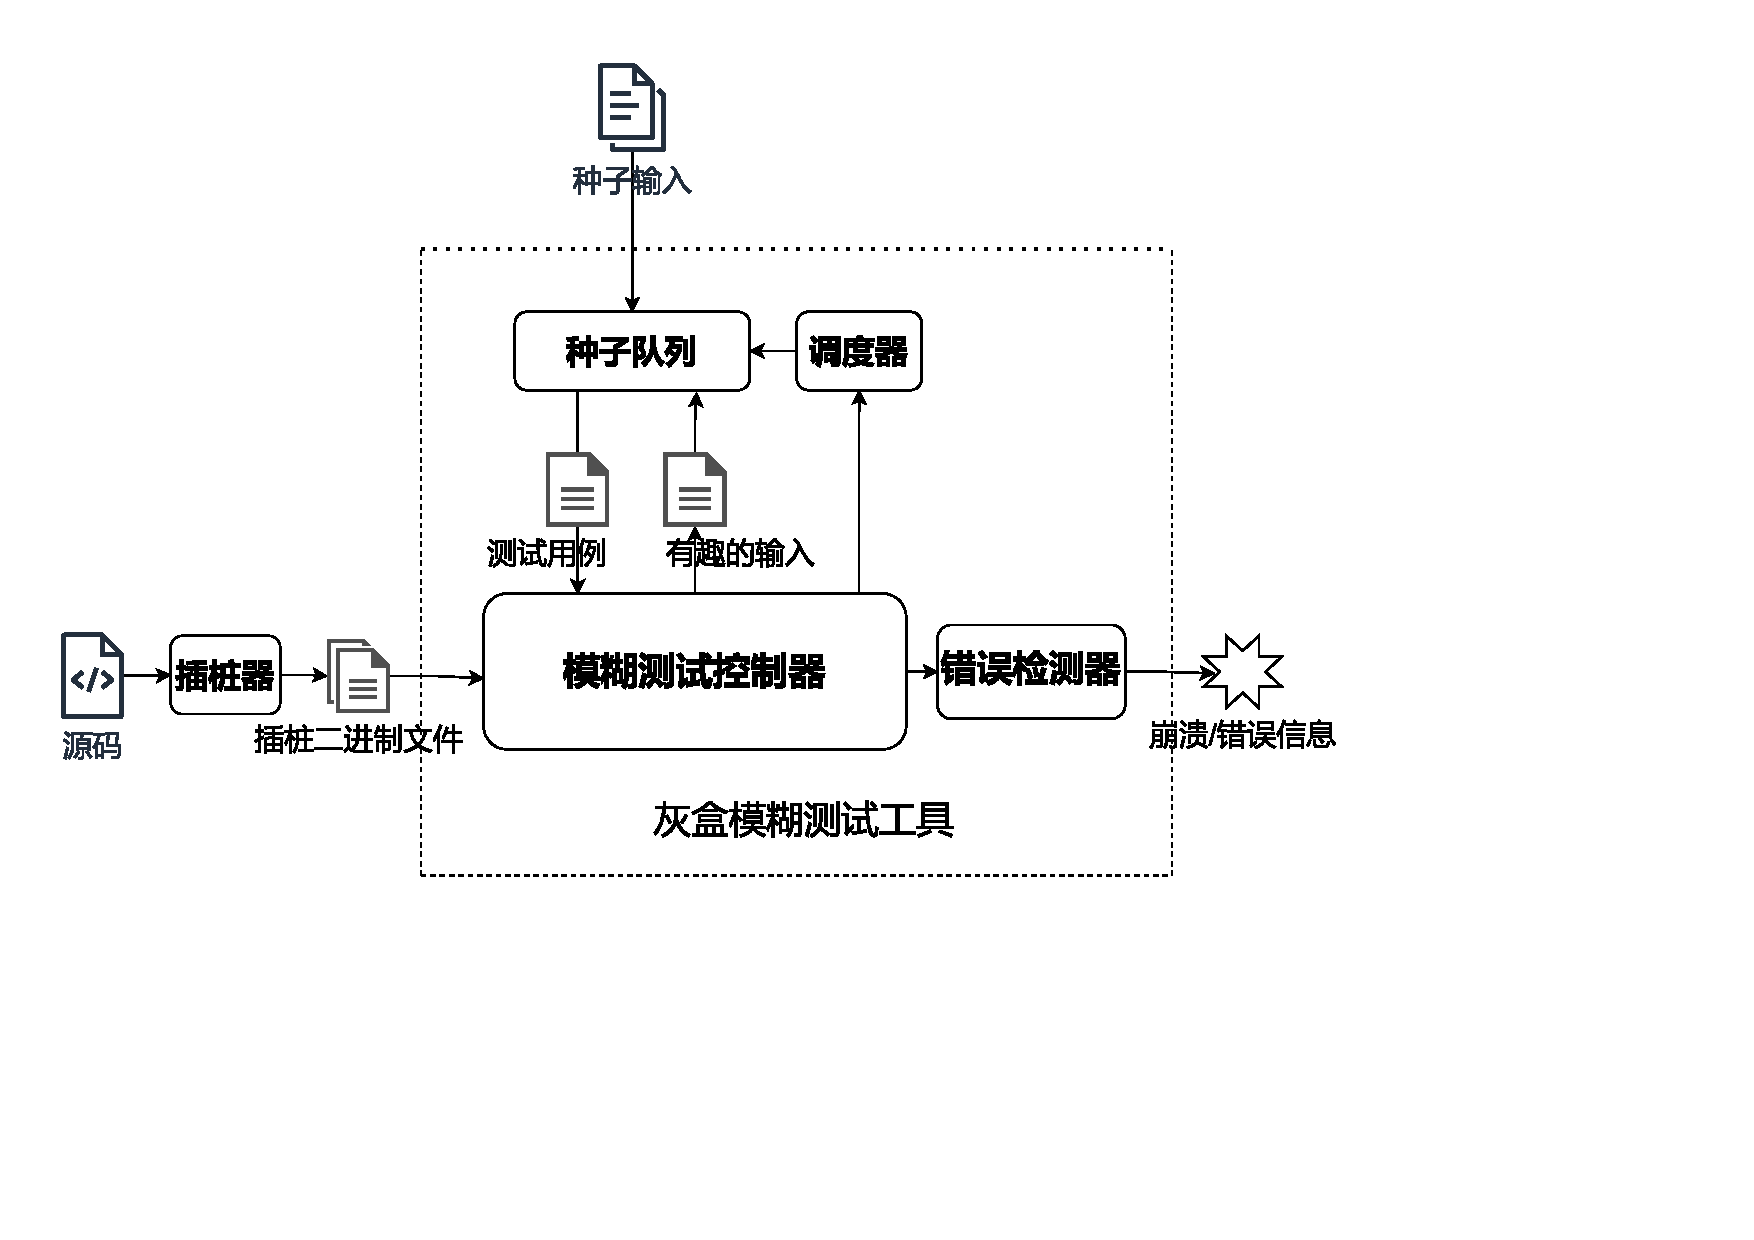
\includegraphics[width=1\textwidth]{pic/GF.pdf}
	\caption{灰盒模糊测试架构}
 	\label{GF}
\end{figure}

由于白盒模糊测试受限于符号执行自身的问题,灰盒模糊测试的方式越来越得到学界重视。这一技术方法介于上述两种技术之间。
通常,灰盒模糊测试工具可以获得被测试程序或其执行的一些内部信息。与白盒模糊测试工具不同,灰盒模糊器不推理
被测试程序的完整语义;相反,其采用对被测试程序执行轻量级静态分析或收集有关其执行的动态信息,例如代码覆盖率,数据流等,
以及配合良好的测试策略,来实现对被测试程序的整体测试。这一技术既综合了白盒模糊测试的优点,亦规避了其效率低下的缺点。

在2013年由Google发布的AFL\cite{AFL}(American Fuzzy Lop)是灰盒模糊测试工具中最重要的一个成果。图\ref{GF}以其为例
展示了一般的灰盒模糊测试工具的基本架构。AFL是一款以覆盖率为导向的模糊测试工具,通过插桩的方法,采集输入数据对应的
边覆盖率,作为模糊测试种子选取的衡量指标,通过设计适当的算法函数,较好的实现了灰盒模糊测试,达到了较高的代码覆盖率。
而对应到一般化算法\ref{alg:fuzzing}中,灰盒模糊测试主要在第7行利用收集到的执行信息(如代码覆盖率,种子发现的新路径等)来
更新算法配置,从而指导测试用例的生成。虽然灰盒模糊测试一般也会在第2行的预处理阶段进行一些静态分析,但相对于白盒模糊测试而言,
其所有的程序分析部分都会在此步或之前完成,采取的是非常轻量级的程序分析技术。具体到AFL来讲,这一步仅仅是识别不同的路径并对
程序进行插桩。

\section{定向模糊测试技术}
前文所述的包括AFL等在内的大部分模糊测试工具的主要是以覆盖率为导向(coverage-based)的模糊测试技术。直觉上来讲,模糊测试工具对程序的代码覆盖率
越大,那么通过模糊测试可以探查到的程序漏洞一般来讲也会更多。故而无论是白盒模糊测试还是以AFL为代表的灰盒模糊测试都是
以扩大代码覆盖率为测试用例生成的主要目标。

而在一些应用场景下,盲目地扩张代码覆盖率未必能取得很好的漏洞检测效果。例如,在对程序的补丁进行测试时,盲目扩大代码的覆盖率
检测正常运行的部分是对资源的浪费。这启发了定向模糊测试(Directed Fuzzing)的思想,与其一味的扩大代码的覆盖率,不如重点检测
特定的代码区域。

而现在意义上的定向模糊测试可以认为是将模糊测试生成的测试用例引导至指定的目标:既可以是指定的代码区域,即源码中的指定行数的代码区域或
二进制文件中的虚拟地址;也可以是指定的特定行为或错误,比如UAF(use-after-free)错误。当然,本文的设计目标是定向覆盖
特定区域,针对特定行为的定向模糊测试技术就不再讨论。

定向模糊测试技术除了上述的补丁测试(Patch Testing)的应用外,还可以用于崩溃重现(Crash Reproduction)、静态分析报告验证(Static Analysis Report Verification)
以及数据流检测(Information Flow Detection)等。
\subsection{白盒定向模糊测试技术}
早期的定向模糊测试是由白盒模糊测试实现的。在2011年由Ma等人提出的定向符号执行\cite{ma2011directed}
(Directed symbolic execution,简称DSE)技术是其中最具代表性的一项工作。

符号执行\cite{king1976select}是一种自动化程序分析技术,它通过对程序输入进行符号化表示并应用约束求解来推导出程序的
所有可能执行路径及其相关状态。在符号执行期间,程序中的每个变量都被表示为一个符号表达式,而不是一个具体值,这可以使分析器在
不运行实际代码的情况下探索程序状态空间的各种可能性。

对于程序的定向覆盖的需求,Ma等人将这一位置可达性问题转换为迭代约束满足问题,也即经典的约束求解问题。通过指定待探测代码区域,
定向符号执行技术利用程序分析来分析所有可到达指定区域的路径,而后通过约束求解生成所有符合执行相应路径的测试用例以来达到对指定区域的覆盖和测试。
Ma等人提出了两种符号执行方式:最短距离符号执行(Shortest-distance symbolic execution,简称SDSE)和调用链后向符号执行
(Call-chain-backward symbolic execution,简称CCBSE)。SDSE是通过过程间控制流图,从起点出发计算可以到达指定区域的最短距离
从而得到合适的路径条件;而CCBSE则是通过从指定区域自后向前执行符号执行,沿着调用链向前查询所有可能到达起点的路径条件。在得到
路径条件后,再通过设置路径约束条件以求解满足条件的生成测试用例。而后测试用例即可依据设定的路径达到指定代码区域,从而实现对
特定区域的测试,也即定向覆盖。

除此以外,无论是结合污点分析技术的BuzzFuzz\cite{ganesh2009taint},还是结合动态符号执行的KLEE\cite{cadar2008klee},都
无外乎是在符号执行引擎中实现,采用探索可行路径的状态空间的方式来实现定向覆盖。

但是这一方式依然具有白盒模糊测试的弊病,那就是对路径条件的探索和对种子生成条件的指引的有效性是以模糊测试的效率为代价的。
当实际被测试程序具有很高的复杂度和规模时,DSE采取的重量级程序分析将面临严重的路径爆炸问题,这也使得实际执行效果并不理想。

\subsection{灰盒定向模糊测试技术}\label{sec:DGF}
由B{\"o}hme等人于2017年提出的AFLGo\cite{bohmeDGF2017}引入了定向灰盒模糊测试(Directed Grey-box Fuzzing, 简称DGF)的概念。
这一工具也正是本文重点研究的架构。相较于繁重的约束求解来解决定向的位置可达性问题,AFLGo采取从另一角度来实现本目标。B{\"o}hme
等人先前于2016年做出的工作\cite{2016Coverage}将模糊测试的路径执行过程建模为马尔科夫链,这为AFLGo的设计提供了思路。

事实上我们知道,一个程序中大多数执行路径是不会被经常执行的,而经常执行的路径往往只占所有路径中的小部分。在AFL的输入构造环节中
种子的能量分配却是平均分配的,这使得那些较少被执行的路径获取得到的种子能量因为相对不足而需要更多的时间才能探索暴露出漏洞。
对此,Böhme等人在他们的工作AFLFast\cite{2016Coverage}中给出的解决办法是将模型糊测试程序建模为对马尔可夫链接状态空间的遍历过程,
将种子变异导致的程序执行路径转移概率,视为马尔可夫链上的状态转移概率。然后通过制定相应的能量分配策略,使得马尔可夫链状态空间的
遍历过程,更倾向于低访问频率的区域,使得能量分配更加合理。通过针对AFLFast和AFL的对比实验表明,这样的能量分配策略使得在同样的
时间中,AFLFast有更多的机会去接近低访问频率的区域从而能够发现比AFL多指数级的崩溃\cite{2016Coverage}。

于是,针对于定向覆盖的问题,AFLGo就将其从位置可达性问题转换为能量分配的优化问题。AFLGo舍弃了繁重的路径条件的求解,而是转而通过
在预处理阶段计算每个基本块与目标位置的距离并将其插桩进入二进制文件,再通过运行时评估每个种子执行路径相对于目标区域的平均距离从而
利用种子的能量调度机制来影响测试用例的生成从而达到定向覆盖的目标。这一机制还会在章节\ref{sec:AFLGo}详细介绍。

现在DGF仍然是模糊测试领域中非常先进的技术。其结合了定向模糊测试和灰盒模糊测试的思想,可以在不需要完全了解被测
系统内部工作原理的情况下,检测出潜在的漏洞和错误。其将大部分的能量分配给重点的代码区域,而不浪费资源于其他无意义的部分,可以更快
更高效地测试代码。同时,相比于白盒定向模糊测试方法,定向灰盒模糊测试可以避免过多地关注程序内部的实现细节,从而
节省生成测试用例的时间成本。

\section{研究动机}
自从定向灰盒模糊测试技术被提出来以来,就有许多相关的研究工作被提出。虽然AFLGo作为定向灰盒模糊测试方向开山之作在该方向的
表现卓有成效,但是其策略在一些方面依然存在着一定的缺陷。后续又涌现出了一批相关的工作,例如Hawkeye\cite{chen2018hawkeye}, 
CDGF\cite{lee2021constraint}, BEACON\cite{huang2022beacon}等。

这些工作指出了AFLGo的诸多不足,例如Chen Hongxu等人认为AFLGo在能量分配上偏向较短的路径,这会导致漏洞的遗漏\cite{chen2018hawkeye};
Gwangmu Lee等人则认为AFLGo在路径上的优化问题处理方式会遗漏目标位置的顺序影响以及不考虑导致崩溃产生的数据条件,从而忽略满足崩溃条件的种子\cite{lee2021constraint};
Heqing Huang则指出AFLGo保留的过多无效路径仍然会影响模糊测试执行的路径以及耗费资源\cite{huang2022beacon}。

这些工作中Chen Hongxu等人的Hawkeye\cite{chen2018hawkeye}对AFLGo的思路沿用最为整体,改进措施较为详细。
但是他们的工作是在其自研的模糊测试框架FOT\cite{chen2018fot}上实现,且该项工具并未开源。这使得对于其成果即灰盒模糊测试的性能
提升较难验证。于是本文的定向算法指标设计主要参考了他们指出的问题,并尝试在开源的AFLGo框架上实现集成指标,以期达到AFLGo的改进。

\section{本章小结}
本章首先详细介绍了模糊测试的一般算法框架,并介绍了模糊测试技术的分类,分别详细区别了黑盒模糊测试,白盒模糊测试以及灰盒模糊测试的不同,一并介绍了
不同技术的特点和相关工具。而后介绍了本文重点关注的定向模糊测试技术,介绍了技术发展初期的定向白盒模糊测试技术原理和相关工具,现在主要流行的
定向灰盒模糊测试技术与典型工作AFLGo。最后,介绍了本文的研究动机和主要参考工作。

\chapter{定向模糊测试策略研究与设计}
\section{AFLGo架构研究}\label{sec:AFLGo}
\begin{algorithm}[H]
	\DontPrintSemicolon
	\SetKwSty{algokeywordsty}
	\SetFuncSty{algofuncsty}
	\SetDataSty{algodatasty}
	\SetArgSty{algoargsty}
	\SetCommentSty{algocmtsty}
	\SetKw{break}{break}
	\SetKw{not}{not}
	\SetKwFunction{graphextractor}{\textsc{GraphExt}}
	\SetKwFunction{bbdistance}{\textsc{DisCalcu}}  
	\SetKwFunction{select}{\textsc{Dequeue}}
	\SetKwFunction{assinenergy}{\textsc{AssinEnergy}}
	\SetKwFunction{mutation}{\textsc{Mutation}}
	\SetKwFunction{execution}{\textsc{Execution}}
	\SetKwFunction{IsIntersting}{\textsc{IsIntersting}}
	\SetKwFunction{evaluateseed}{\textsc{SeedDis}}
	\SetKwFunction{sortinsert}{Enqueue}
	\SetKwData{crashseeds}{$\seeds^\prime$} 
	\SetKwData{seedqueue}{$\textit{SeedQueue}$}  
	\SetKwData{Graph}{$\textit{Graphs}$}  
	\SetKwData{BBdis}{$\textit{BBdistance}$} 
	\SetKwData{newseed}{$\seed^\prime$}   
	\SetKwData{energy}{$\textit{e}$}
	\SetKwData{trace}{$\textit{trace}$} 
	\SetKwData{distance}{$\textit{distance}$}   
	\KwIn{\seeds\tcp{a finite set of seeds}}
	\KwIn{\targets\tcp{a finite set of targer sits}} 
	\KwOut{\crashseeds \tcp{a finite set of buggy seeds}}
	$\crashseeds\gets \varnothing$\; 
	$\seedqueue \gets \seeds$\;
	\Graph $\gets \graphextractor{\sourcecode}$\;
	\BBdis $\gets \bbdistance{\targets,\Graph}$\;
	\While {$!siganl \land \currtime < \timeout$}{
	  \seed$\gets \select{\seedqueue}$\;
	  $\trace \gets \execution{\seed}$\; 
	  $\distance \gets \evaluateseed{\trace, \BBdis} $\;
	  \energy $\gets \assinenergy{\seed, \currtime, \distance}$\;
	   \For{$\textit{i}\gets 1$ \KwTo $\energy$}
	   {
		$\newseed \gets \mutation{\seed}$\;      
		\lIf{\newseed crashes}{$\crashseeds \gets \crashseeds \cup \newseed $}
		\lIf{\IsIntersting{\newseed}}{    
			$\sortinsert{\newseed,\seedqueue} $ 
		}
	   }
	}
	\Return{\crashseeds}\;
	\caption[short]{定向灰盒模糊测试算法}\label{alg:DGF} 
\end{algorithm} 
\vspace{6pt}
本文以AFLGo为主要研究对象,且主要改进及算法实现均在AFLGo上实现,故本节将详细介绍AFLGo的基本架构。

算法\ref{alg:DGF}展现了AFLGo的基本执行流程。可以看到与算法\ref{alg:fuzzing}的基本结构相同。AFLGo采取的算法配置包括:种子队列,
种子分配能量以及种子执行路径的距离。而AFLGo主要的修改可以分为在预处理阶段阶段和运行阶段两个阶段。

在算法\ref{alg:DGF}的第3行和第4行是算法的预处理阶段。在这一阶段,AFLGo通过先进行一次插桩编译计算出被测试程序的调用图(Call Graph,简称CG)
和每个函数对应的控制流图(Control-flow Graph,简称CFG),这一步是算法\ref{alg:DGF}的第3行实现。再通过利用提供的目标(即源码中对应的代码行号)
识别出目标代码所在的函数(Target Function),在CG中利用迪杰斯特拉最短路径算法得到每个函数到达目标函数的最短距离。而后结合对应每个函数的CFG计算
函数中的基本块到目标代码所在基本块(Target Basic Block)的距离。这一步是在算法\ref{alg:DGF}的第4行实现。此后,AFLGo会再执行一次插桩将代码
距离植入每一个基本块。

在算法\ref{alg:DGF}的第7、8和9行是算法的算法配置更新阶段。针对种子池中的所有输入种子,AFLGo都会将其执行一遍,并收集执行过程中种子 路径的平均距离。
这一步由算法的第7、8行完成。而后,算法会依据种子的距离以及算法已执行的时间,向种子分配能量(注意,在ALFGo中将种子的能量定义为由种子生成的
测试用例数量)。而后通过利用模拟退火的优化方式对种子分配能量,来引导测试用例更多的倾向于探测覆盖指定区域。

\subsection{距离计算机制}
\begin{figure}[htbp]
	\centering
	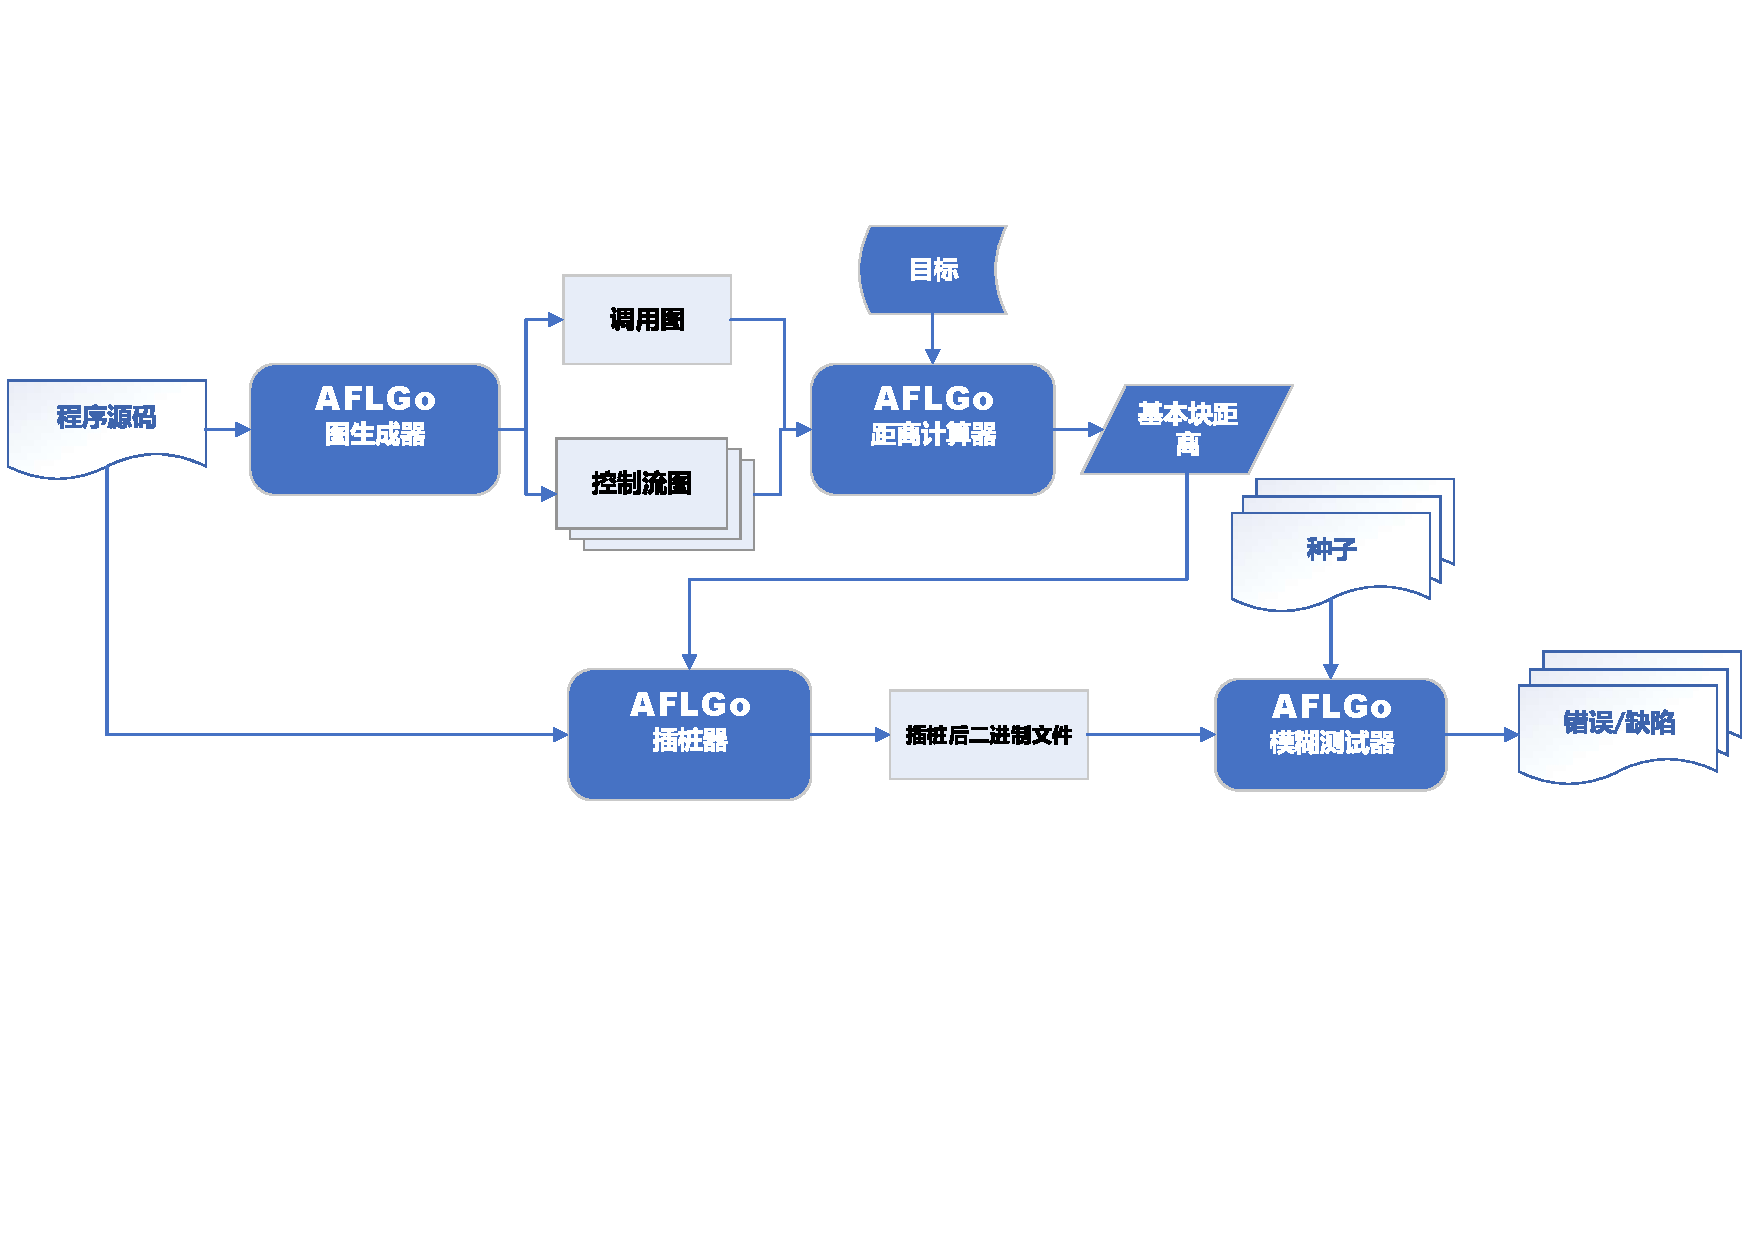
\includegraphics[width=1\textwidth]{pic/AFLGo.pdf}
	\caption{AFLGo基本框架}
 	\label{pic:AFLGo}
\end{figure}

图\ref{pic:AFLGo}展示了AFLGo的基本框架。与图\ref{GF}所展示的灰盒模糊测试的基本框架相比,AFLGo做出较大改变的就是预处理的插桩部分。
AFLGo利用LLVM的pass\cite{Pass}对程序的源码实现了编译器级别的分析和插桩。利用AFLGo的图生成器,AFLGo将得到程序的CG和CFG,这将用于
参与计算AFLGo的函数级距离和基本块级目标距离。此外,可以根据提供的源码行号指定的目标得到目标代码所在的目标函数集$T_f$和目标基本块集$T_b$。
而后,根据CG就可以计算函数级目标距离。

函数级距离 $d_f(n, n')$ 定义为调用图CG中函数 $n$ 和 $n'$ 之间最短路径上的边数。而函数$n$与目标函数 $T_f$ 
之间的函数级目标距离 $d_f (n,T_f) $则被定义为 $n$ 与任何可达目标函数 $t_f \in T_f$ 之间函数距离的调和平均值:
 \begin{equation}\label{eq:fdis}
	d_f(n,T_f)=\left\{ \begin{aligned}
		&\text{undefined} , &\text{if } R(n,T_f)=\varnothing \\
	   [&\sum\limits_{t_f\in R(n,T_f)} d_f(n,t_f)^{-1}]^{-1} , &\text{otherwise} 
   \end{aligned}
   \right.
 \end{equation}
式\ref{eq:fdis}中$R(n,T_f)$为从函数$n$出发可达的目标函数集$T_f$中的所有目标函数$t_f$的集合。注意,AFLGo是支持
多个目标的,这也意味着目标函数可能不止一个。关于这里采用调和平均的计算方式,图\ref{pic:diff}展示了一个例子。在图中
(a)采用了算数平均,而(b)采取了调和平均。当有多个目标函数时,在调用图中利用算数平均计算函数间目标距离无法很好地区分
当到达不同目标函数的最短路径总和恰好相等时,究竟哪个函数离其中某个目标函数更近一点的情况。

\begin{figure}[htbp]
	\centering
	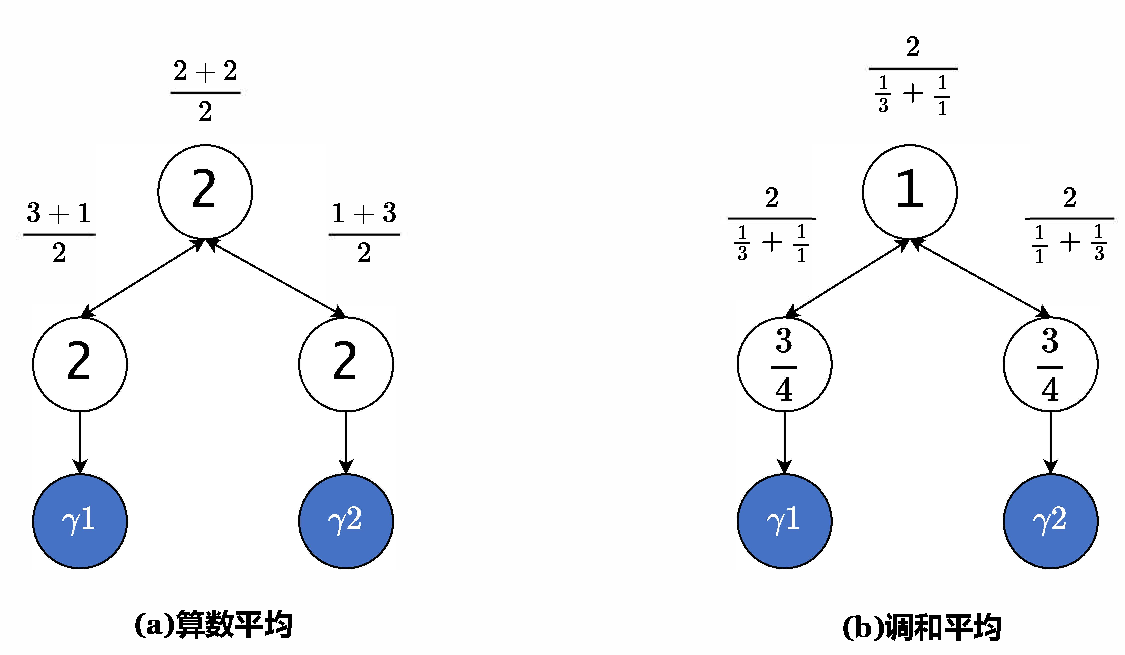
\includegraphics[width=0.6\textwidth]{pic/diff.pdf}
	\caption{算数平均与调和平均的差异}
 	\label{pic:diff}
\end{figure}

基本块级目标函数距离则要依托函数级目标距离来参与计算。基本块级目标距离确定了从当前基本块到目标基本块的距离,
并且考虑了调用函数的函数级目标距离。基本块级距离决定了一个函数的CFG中任意两个基本块之间的距离。因此,将基本块级距离
$d_b(m_1, m_2)$ 定义为函数$i$的控制流图$G_i$中基本块$m_1$和$m_2$ 之间最短路径上的边数。设$N(m)$为基本块 $m$的一个调用
函数集,且有$\forall n \in N (m)$都有$R(n,T_f) \neq \varnothing$。设 $T$是 $G_i$中一个基本块集,且有$\forall m \in T$ 
都有$N(m)\neq \varnothing$。请注意,目标基本块$T_b$不一定需要存在于当前CFG $G_i$中,但 $G_i$中可能存在可以沿着调用函数链到达
包含目标基本块$T_b$的目标函数的基本块集$T$。那么我们可以定义基本块$m$到目标基本块的$T_b$的基本块级目标距离$d_b(m,T_b)$为:
\begin{equation}\label{eq:bbdis}
	d_b(m,T_b)=\left\{ \begin{aligned}
		&0 ,&\text{if } m \in T_b \\
		&c \cdot \min \limits_{n\in N(m)}(d_f(n,T_f)) , &\text{if } m \in T \\
	   [&\sum\limits_{t\in T} (d_b(m,t)+d_b(t,T_b))^{-1}]^{-1} , &\text{otherwise} 
   \end{aligned}
   \right.
 \end{equation}
式\ref{eq:bbdis}中的$c$为常数,在实际中取$c=10$。

在通过利用CG和每个函数的CFG计算得到程序中所有基本块的基本块级目标距离$d_b(m,T_b)$后,AFLGo就将该数值通过第二次对程序的编译插桩
进所有基本块中。至此,AFLGo的预处理阶段就结束了。

\subsection{能量调度机制}
在经过了预处理之后的二进制文件在被AFLGo测试时会收集执行测试的每个种子$s$的目标距离$d(s,T_b)$。设种子$s$的执行 路径为$\xi (s)$,那么我们可以定义
衡量种子执行与目标基本块$T_b$远近的种子目标距离$d(s,T_b)$为:
\begin{equation}\label{eq:sdis}
	d(s,T_b)=\frac{\sum\limits_{m \in \xi (s)}d_b(m,T_b)}{| \xi(s)| }
\end{equation}
有了种子的目标距离,也就很好相应的定义种子的归一化目标距离用以作为种子能量分配调度的评判指标。针对种子池$S$中所有种子,
可以在种子$s'\in S$执行时计算种子$s'$对应的归一化目标距离:
\begin{equation}\label{eq:sndis}
	\widetilde{d}(s,T_b)=\frac{d(s,T_b)-\text{minD}}{\text{maxD}-\text{minD}} \in [0,1]
\end{equation}
其中
\begin{equation}
	\text{minD}=\min\limits_{s'\in S}[d(s',T_b)] ,\\
	\text{maxD}=\max\limits_{s'\in S}[d(s',T_b)] 	
\end{equation}

AFLGo的整体能量调度思路就是通过给种子目标距离更近的种子分配更多的能量,从而实现对目标的导向覆盖。这一思路来源于对模糊测试的马尔科夫链建模,这部分
已经在章节\ref{sec:DGF}做了详细的介绍。在AFLGo中引入了模拟退火机制来进一步增加对能量调度的导向性,以期处理探索-开发问题。

模拟退火算法是一种基于概率思想的全局优化算法,常用于解决组合优化问题。该算法基于统计力学中的退火过程,通过随机搜索
来避免陷入局部最优解,从而寻找全局最优解。与经典的随机搜索方式相比,模拟退火的调度方式会以一定的概率接受较差的解,而这
使得模拟退火调度方式有跳出局部最优解达到全局最优解的可能性。接受较差解的概率由参数“温度”控制,随着时间的推延,温度逐渐下降,
能量调度也就越发降低接受较差解的可能性。随着温度最终的降低,模拟退火将找到一个全局的近似最优解。

在AFLGo中,初始温度$T=T_0=1$。温度$T=1$时,AFLGo对能量的调度更倾向于平均分配,不受种子目标距离的影响。此时是处于AFLGo的
开发阶段;而当$T=0$时,AFLGo对于能量的调度则更倾向于梯度下降,将最多的能量分配给种子目标距离更小的种子,而将较少的能量
分配给种子目标距离更大的种子。此时处于AFLGo的开发阶段。

AFLGo采取指数型的冷却调度:
\begin{equation}
	T=T_0 \times \alpha^k	
\end{equation}
其中$\alpha$是一个小于1的常量,通常介于0.8到0.99之间;$k$是当前温度循环次数。由于温度决定了能量分配的策略,于是将$T_k=0.05$
设置为温度阈值。当$T_k \leq 0.05$时,算法不再接受更差的解,进入开发阶段。

将模糊测试已经执行的时间$t$作为调整温度循环$T_k$的参数,公式如下:
\begin{equation}\label{eq:tk}
	\frac{k}{k_x}=\frac{t}{t_x}	
\end{equation}
其中$k_x$是温度到达阈值$T_k$时的温度循环次数;$t_x$是此时模糊测试已经执行的时间。在AFLGo中,达到温度阈值时模糊测试已经执行的时间$t_x$由测试者预设,
是已知量。

结合温度阈值$T_k=0.05=\alpha^{k_x}$,那么要想计算某运行时刻$t$和温度$T$的关系。只需带入式\ref{eq:tk},有:
\begin{equation}\label{eq:t}
	T=\alpha^k=\alpha^{\frac{t}{t_x}\times\frac{\log(0.05)}{\log(\alpha)}}=20^{-\frac{t}{t_x}}
\end{equation}

接下来,使用温度结合种子目标距离来进行能量调度。对给定的种子$s$,可以定义其被分配的能量分配因子$p(s)$为:
\begin{equation}\label{eq:energy}
	p(s)=(1-\widetilde{d}(s,T_b))\cdot(1-T)+0.5T
\end{equation}
式中的$\widetilde{d}(s,T_b)$即由式\ref{eq:sndis}计算得到;当前温度$T$由式\ref{eq:t}计算得到。

\begin{figure}[htb]
	\centering
	\subfigure[能量分配与种子目标距离的的关系]{
		\begin{minipage}[b]{0.47\textwidth}
			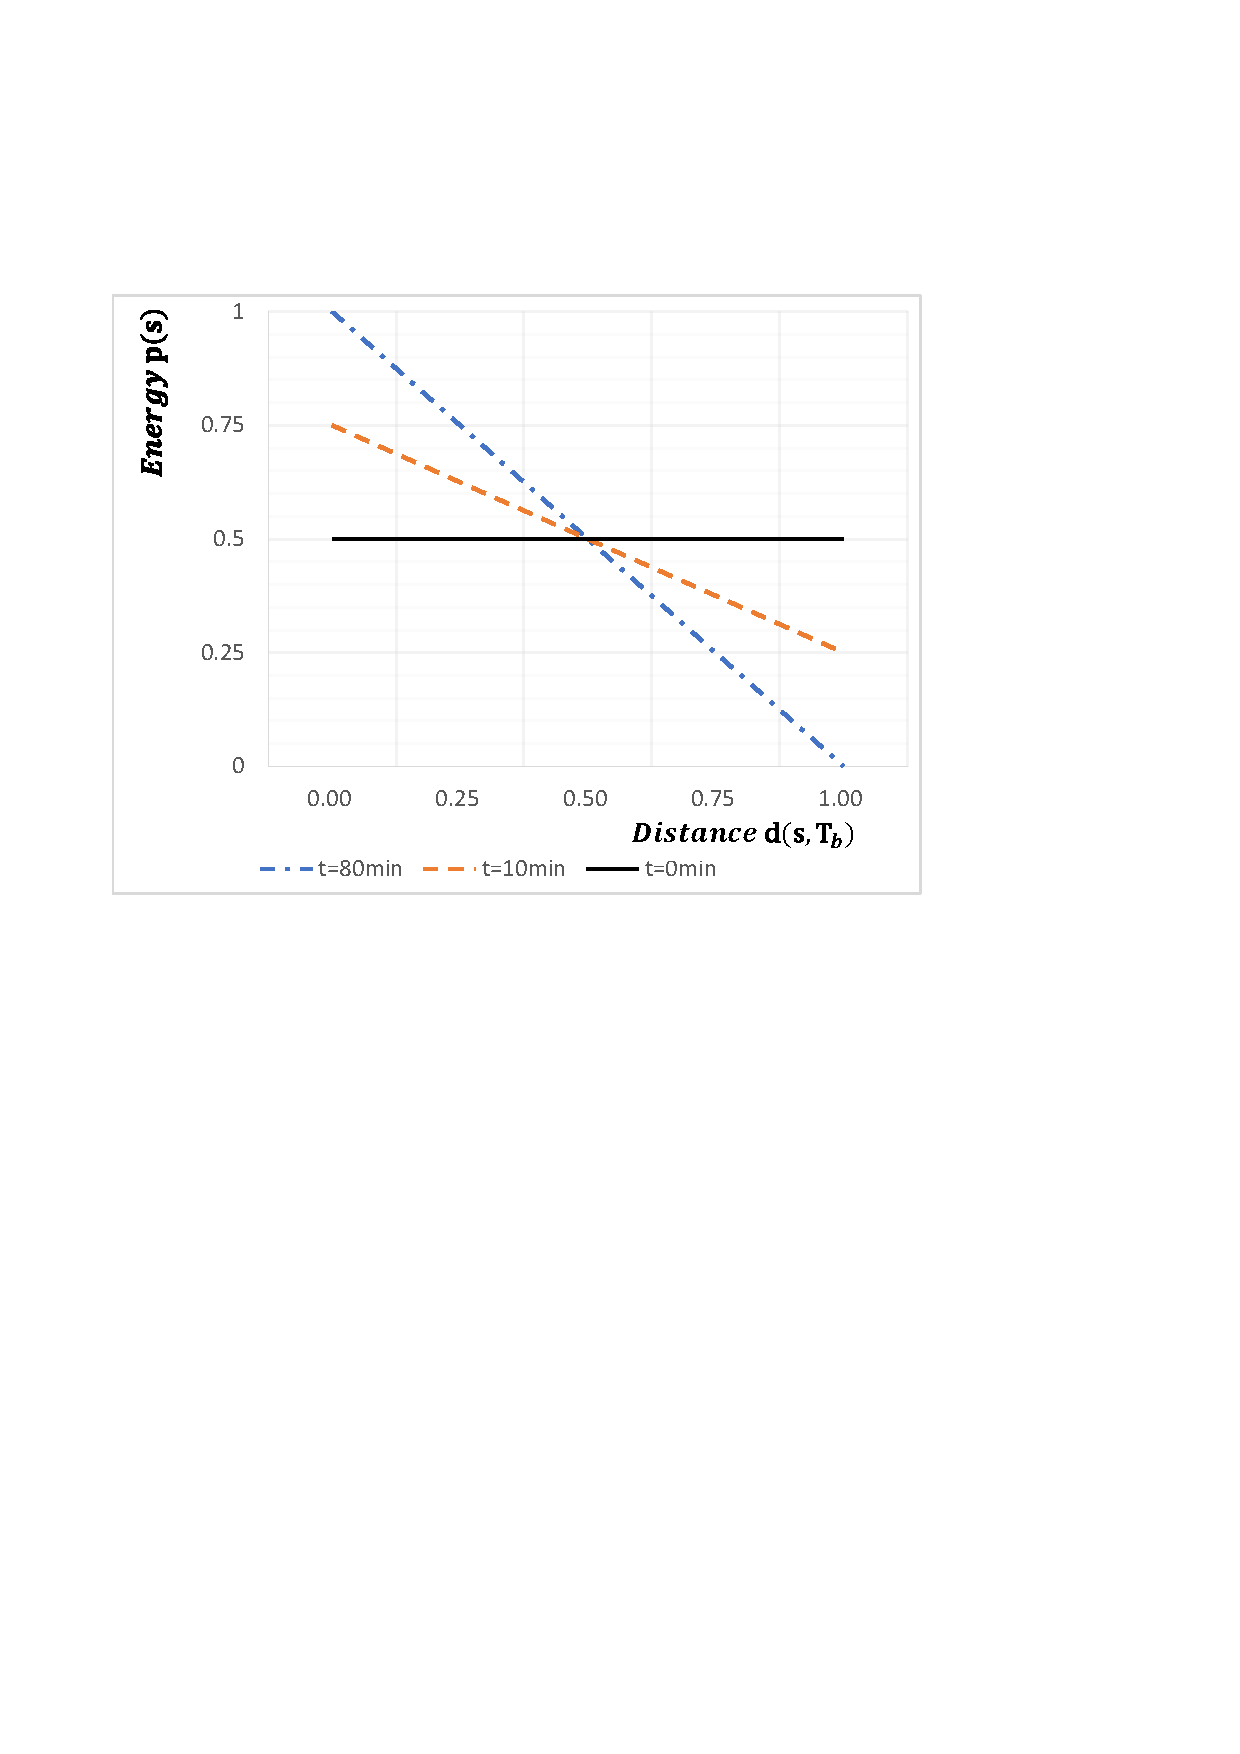
\includegraphics[width=1\textwidth]{dis.pdf}
		\end{minipage}
		}
	\subfigure[能量分配与执行时间的关系]{
		\begin{minipage}[b]{0.47\textwidth}
		 	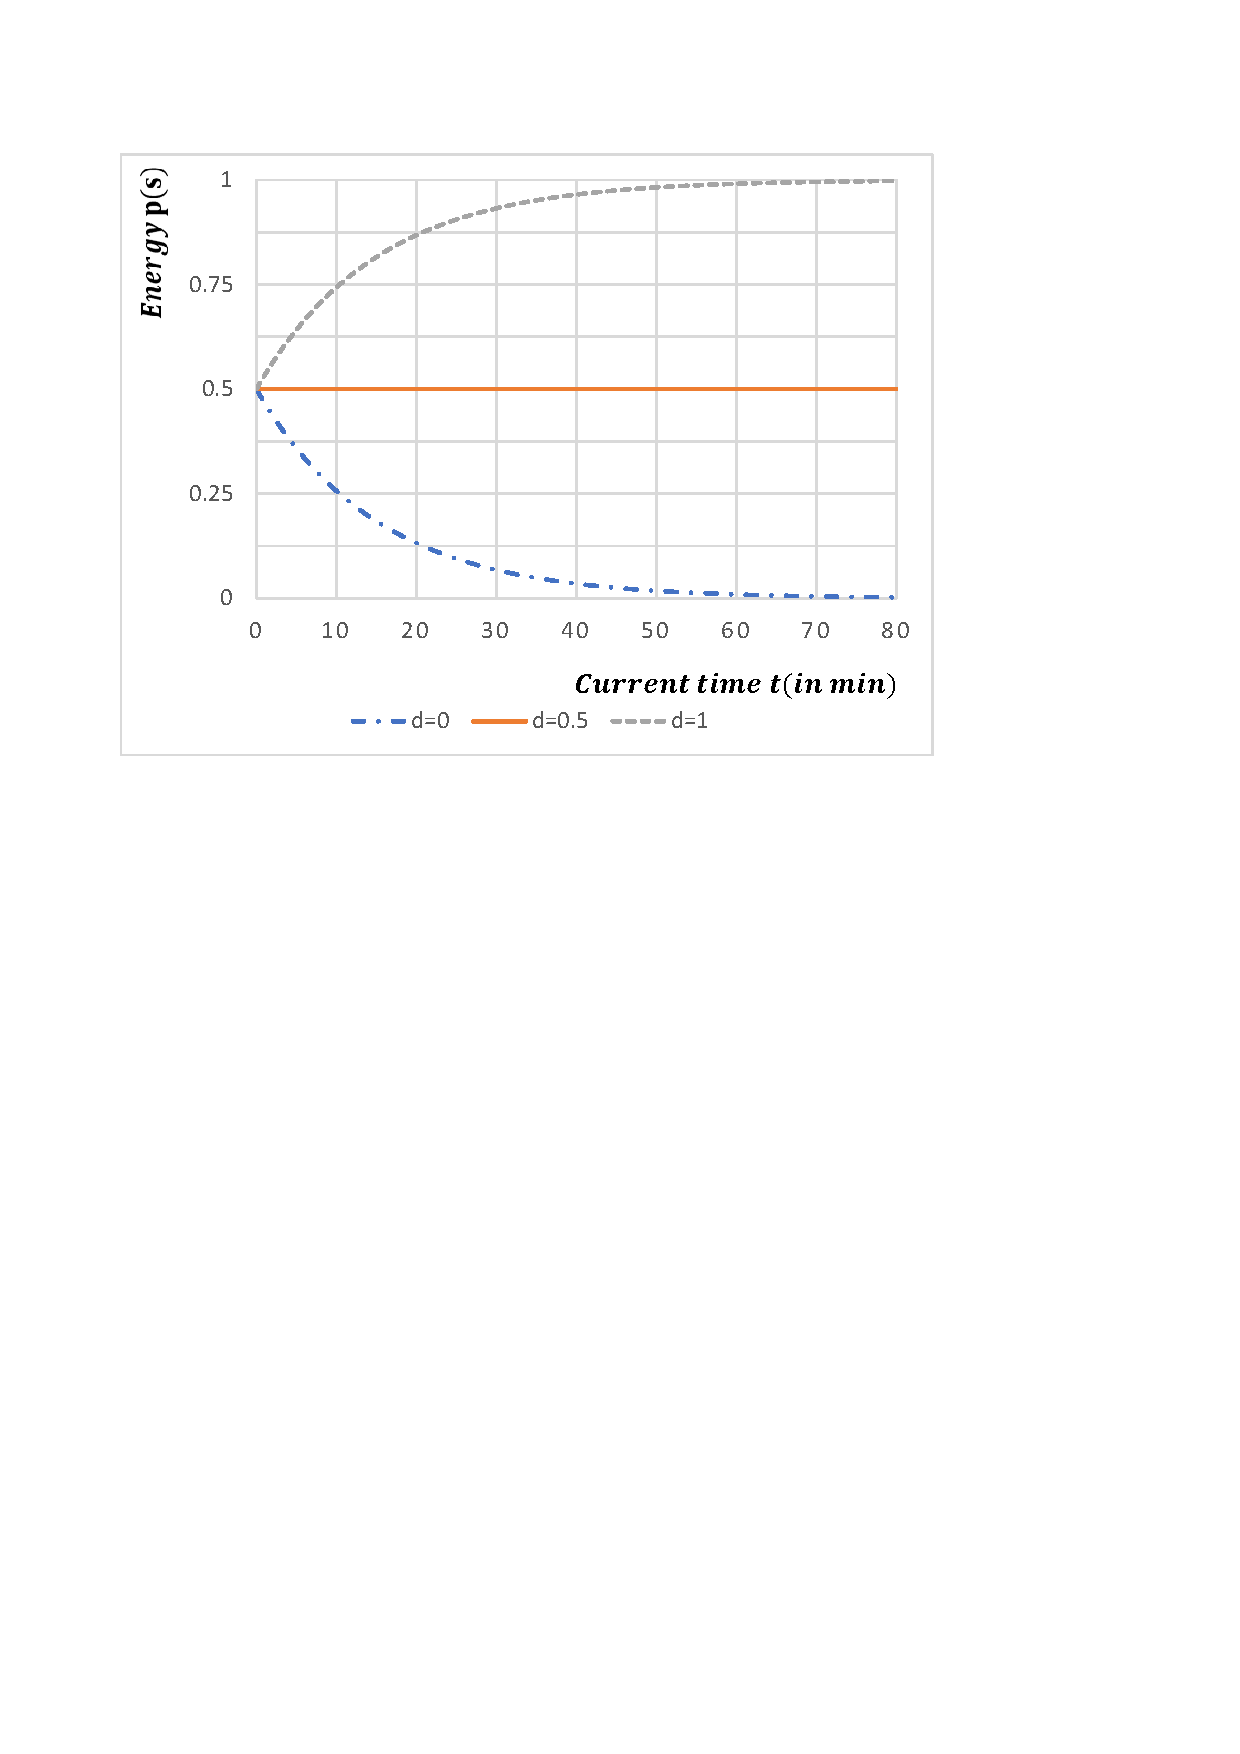
\includegraphics[width=1\textwidth]{dis2.pdf}
		\end{minipage}
		} 
	\caption{模拟退火能量分配方式}
 	\label{pic:dis}
\end{figure}

则最终的种子被分配能量$\hat{p(s)}$为:
\begin{equation}
	\hat{p(s)}=p_{afl}(s)\cdot 2^{10\cdot p(s)-5}	
\end{equation}
式中的$p_{afl}(s)$是原有框架AFL为种子赋予的原始能量。

图\ref{pic:dis}展示了在设置时间阈值$t_x=45$时模拟退火调度下种子能量与归一化种子目标距离$d(s,T_b)$和模糊测试已经执行时间$t$之间的
关系。其中(a)图展现了能量分配机制在不同的已执行时间条件下针对不同的归一化种子目标距离的种子的能量分配方式;(b)图展示了
不同的归一化种子目标距离的种子随着执行时间的增加分配能量的变化。

\section{定向适应度指标设计}
AFLGo的能量调度策略以及设计方式奠定了DGF的基本流程框架。但是,在DGF关于距离的定义机制应该是公平且不带有偏见性的。也即,
DGF应该有一个很好的基于距离的机制,可以通过考虑到目标的所有执行路径并避免对某些执行路径的偏见来指导定向模糊测试。此外,作为灰盒模糊测试
,DGF应该在静态分析的开销和实用程序之间取得平衡。

出于以上原则,实际上上述AFLGo的距离设计和能量调度的机制会具有一定的偏见性。这也是本文针对AFLGo设计改进的基础,将在以下小节分别阐述。
\subsection{距离定义}\label{sec:disredefine}
让我们回到AFLGo对于函数级距离的定义并重新审视它:函数级距离 $d_f(n, n')$ 定义为调用图CG中函数 $n$ 和 $n'$ 之间最短路径上的边数。
事实上这一定义中包含了一项默认信息,即从一个函数$n$到另一个函数$n'$的单位距离是调用图中相邻函数之间的一条边,即单位“1”.

这样的默认条件只考虑了函数间的调用关系。我们再回到AFLGo对模糊测试过程的马尔科夫链建模过程:种子变异导致的程序执行路径转移概率,
为马尔可夫链上的状态转移概率。那么函数间的函数级距离事实上也应该反映函数间互相调用(状态转移)的概率。

\begin{figure}[htb]
	\centering
	\subfigure[code1]{
		\begin{minipage}[b]{0.35\textwidth}
			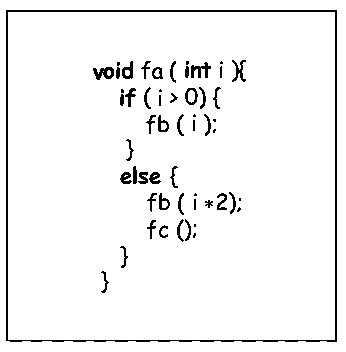
\includegraphics[width=1\textwidth]{code1.pdf}
		\end{minipage}
		}
	\subfigure[code2]{
		\begin{minipage}[b]{0.35\textwidth}
		 	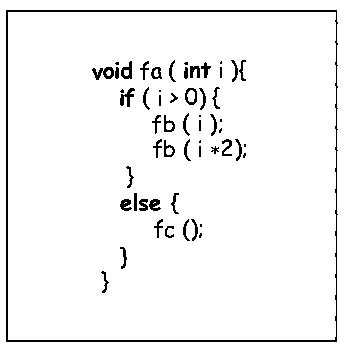
\includegraphics[width=1\textwidth]{code2.pdf}
		\end{minipage}
		} \\
	\subfigure[code1-cfg]{
		\begin{minipage}[b]{0.3\textwidth}
			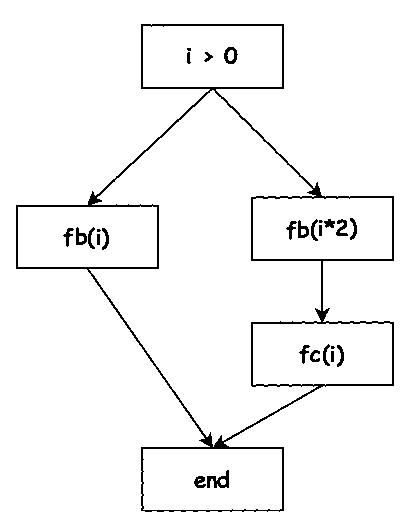
\includegraphics[width=1\textwidth]{excfg1.pdf}
		\end{minipage}
		}
	\subfigure[cg]{
			\begin{minipage}[b]{0.25\textwidth}
				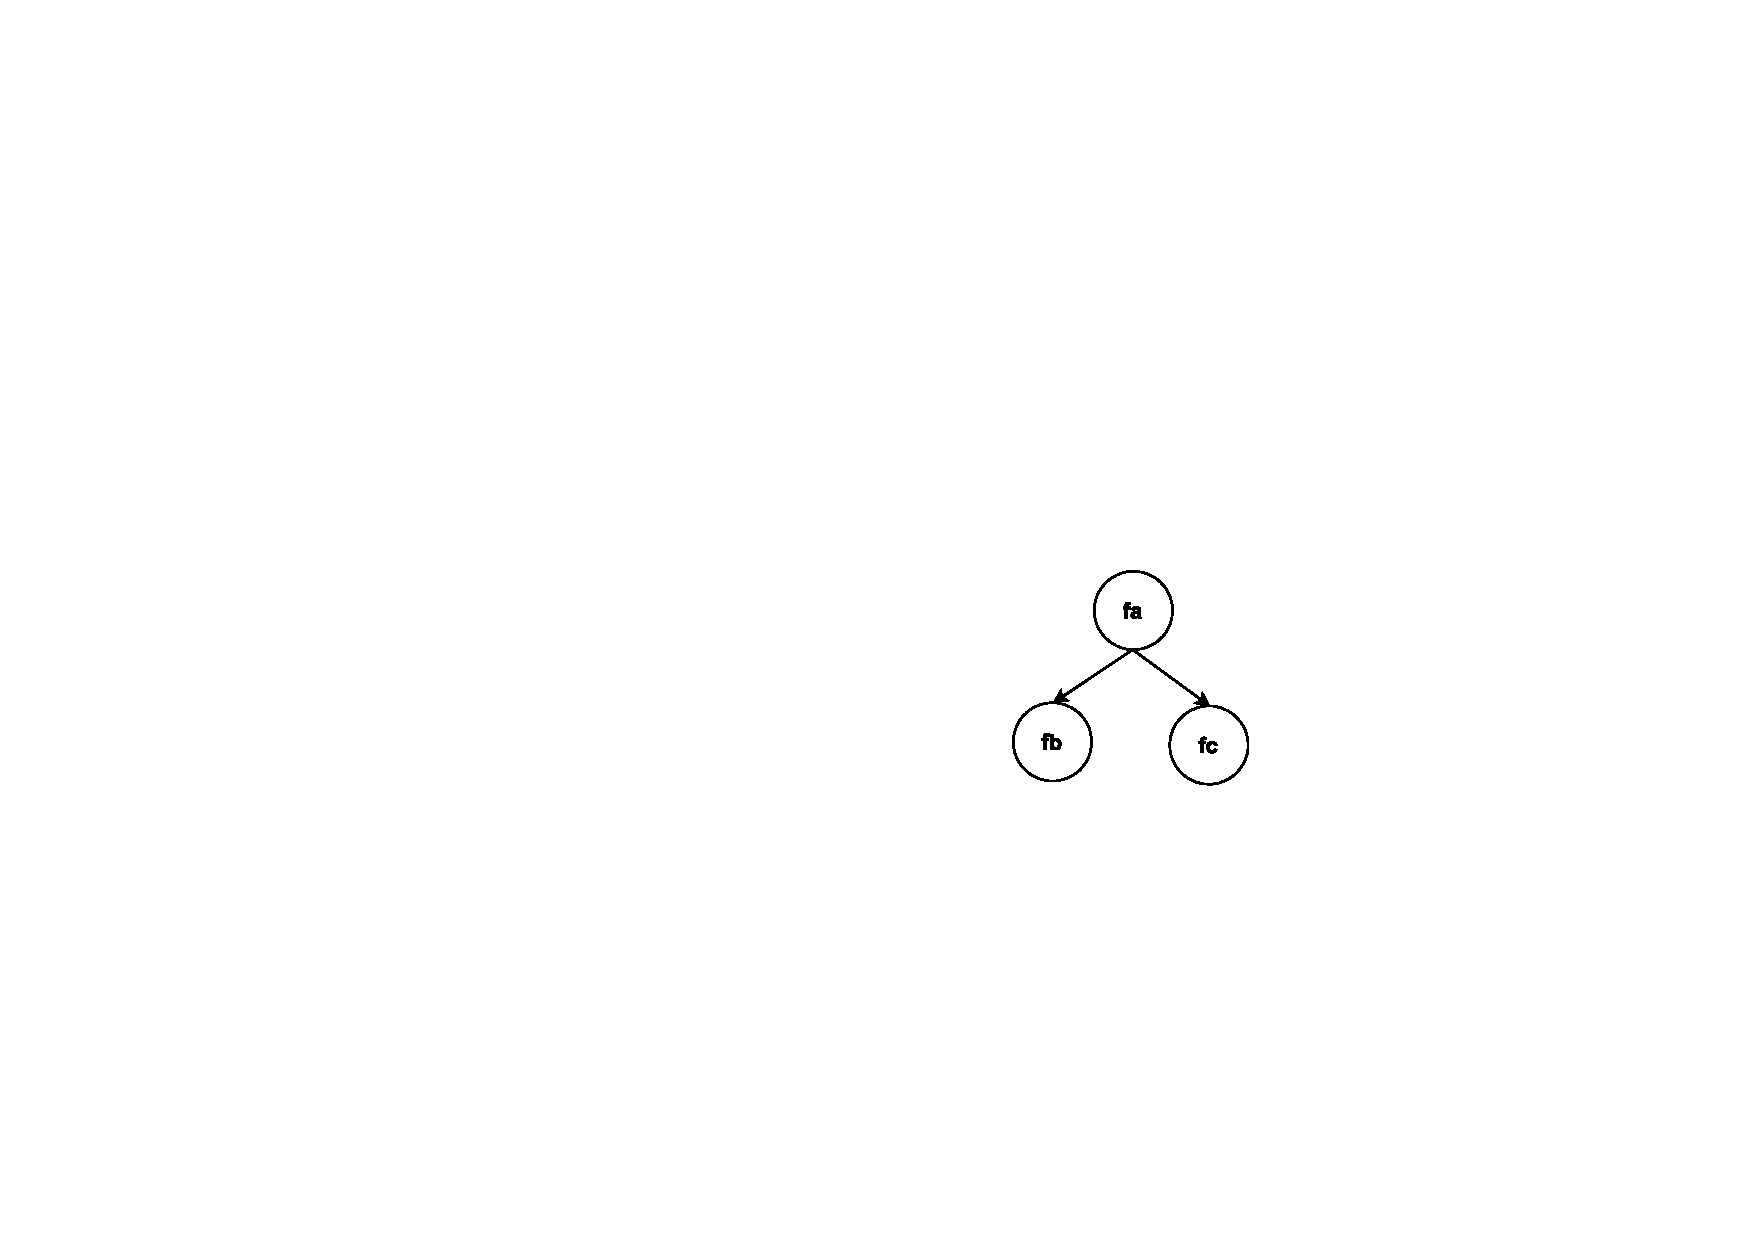
\includegraphics[width=1\textwidth]{excg.pdf}
			\end{minipage}
			}	
	\subfigure[code2-cfg]{
		\begin{minipage}[b]{0.3\textwidth}
		 	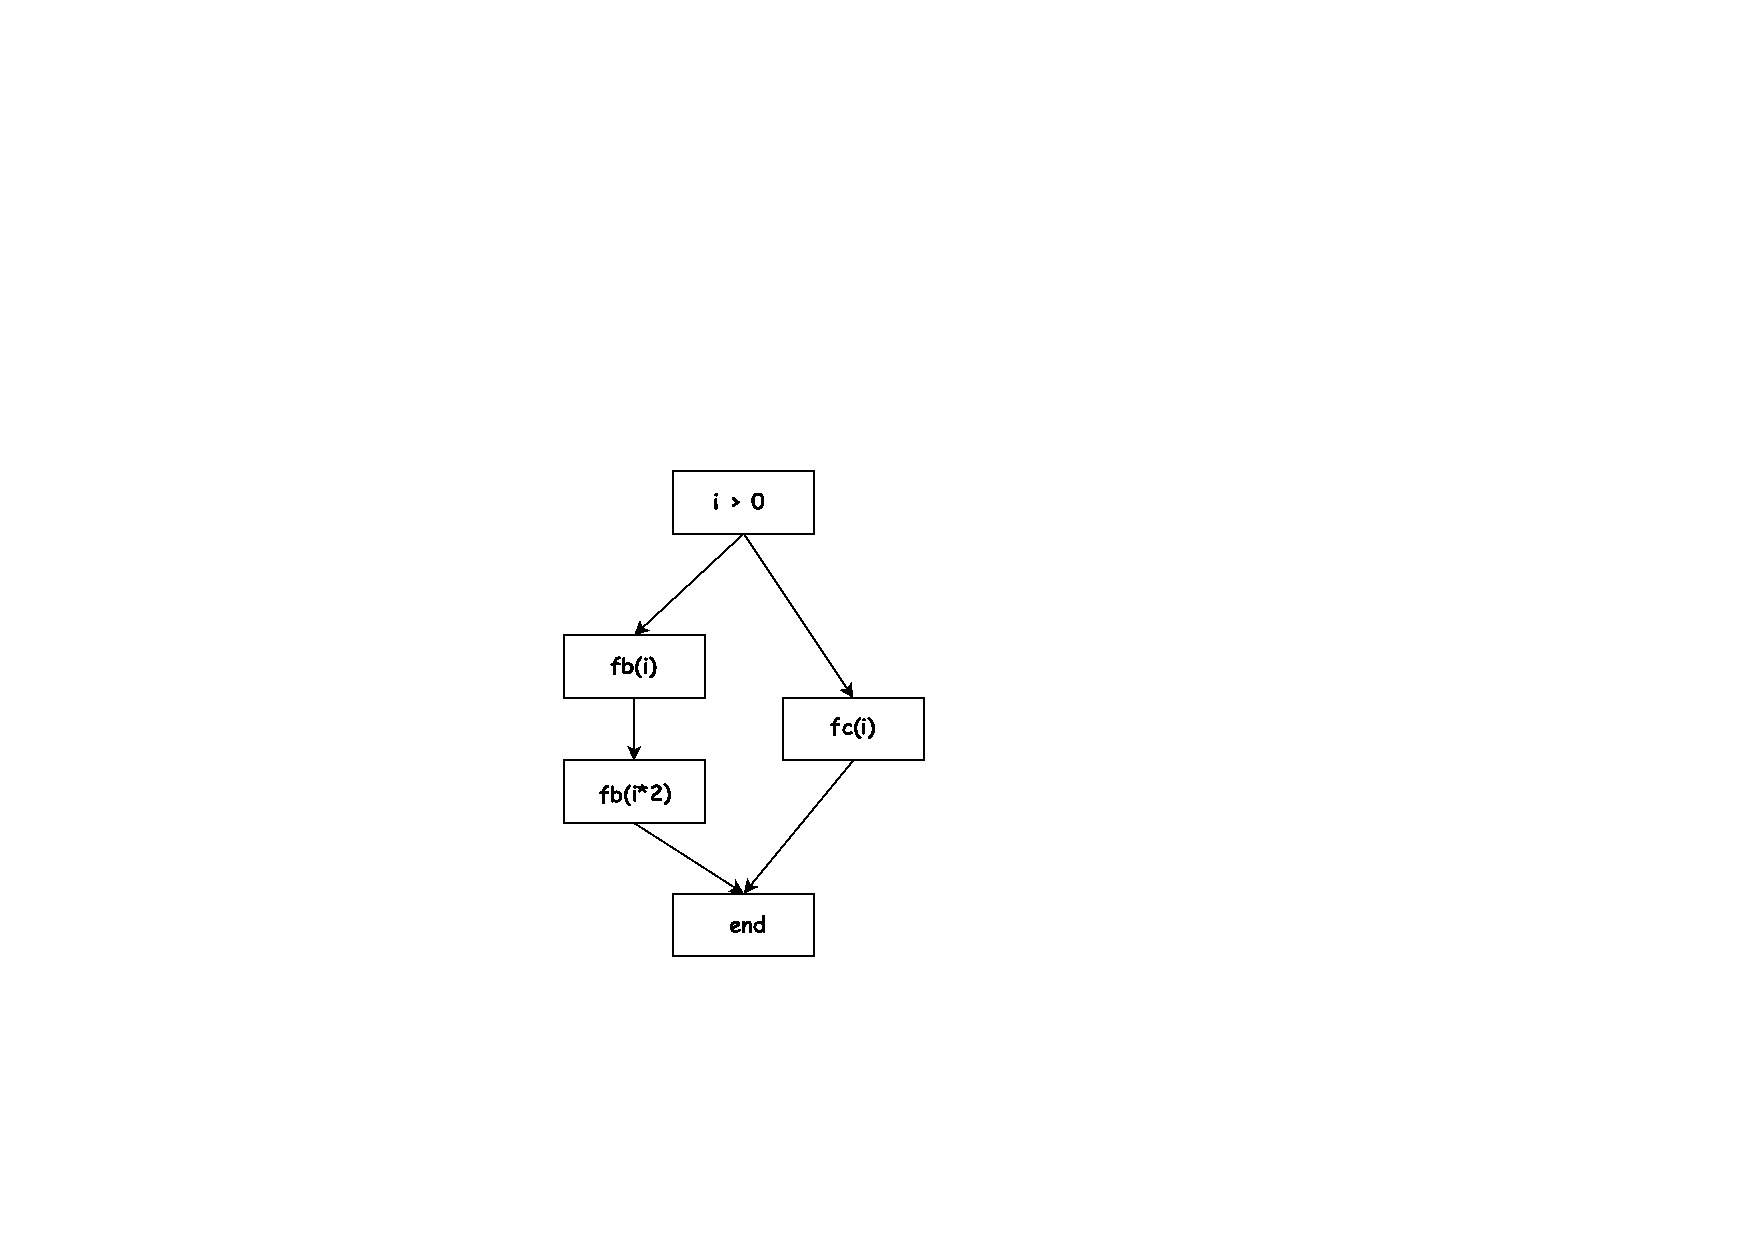
\includegraphics[width=1\textwidth]{excfg2.pdf}
		\end{minipage}
		} 	
	\caption{代码示例}
 	\label{pic:code}
\end{figure}

图\ref{pic:code}展现了这样的一个例子:(a)和(b)是两个不同的函数调用代码,但是它们的调用图CG都如(d)图所示一样。但是如果仔细追究
其所对应的控制流图CFG,也即(c)和(e)时,可以知道在这个两个代码示例中,函数$fa$对函数$fb,fc$的调用概率(状态转移概率)是不同的。
在(a)的情况下$fa$必然会调用$fb$,而不一定调用$fc$;在(b)的情况下$fa$并不一定会调用$fb$。但是仅凭(d)中的调用图CG是无法
反映这样的区别的,也即这两种状况下被计算的得到的函数级距离是相同的。我们期望的理想状态应该是在(a)的情况下,$fa \to fb$的距离应当
小于(b)情况下的$fa \to fb$的距离。

这就使得我们得重新定义一个更精确的函数级距离。因此,我们采取使用两个额外的指标来增加由调用函数(称作“caller”)和被调用函数(称作“callee”)
之间的直接调用关系定义的距离。
\begin{enumerate}[label=(\arabic*)]
	\item 给定调用函数caller中针对某个被调用函数callee的调用点的出现次数$C_N$。
	被调用函数callee的出现次数越多,就越有可能在执行时被调用函数caller调用,
	从而使调用函数caller到被调用函数callee之间的距离变小。为了显示这一效果,定义一个因子:
	\begin{equation}\label{eq:factor1}
	\Phi (C_N)=\frac{\phi \cdot C_N+1}{\phi \cdot C_N}
	\end{equation}
	其中$\phi$为常量,一般取$\phi=2$。
	\item 调用函数caller中至少包含一个被调用函数callee调用点的基本块的个数$C_B$。
	随着调用函数中更多分支(或者说,基本块)具有调用点,也就意味着更多不同的执行路径将包括被调用函数。
	为了显示这一效果,定义一个因子:
	\begin{equation}\label{eq:factor2}
	\Psi (C_B)=\frac{\psi \cdot C_B+1}{\psi \cdot C_B}
	\end{equation}
	其中$\psi$为常量,一般取$\psi=2$。	
\end{enumerate}

现在,有了这两个影响因子,我们可以重新定义函数级距离$d(f_1,f_2)$:
\begin{equation}\label{eq:ffdis}
	d(f_1,f_2)=\Psi (f_1,f_2)\cdot \Phi (f_1,f_2) 
\end{equation}
注意这里的$f_1,f_2$是调用函数与被调用函数的关系。我们再以图\ref{pic:code}中的例子来做验证。
对于(a)中的情况,
$d(fa,fb)=\frac{2\cdot 2+1}{2\cdot 2} \cdot \frac{2\cdot 2+1}{2\cdot 2} = 1.56$,
$d(fa,fc)=\frac{2\cdot 1+1}{2\cdot 1} \cdot \frac{2\cdot 1+1}{2\cdot 1} = 2.25$。
对于(b)中的情况,
$d(fa,fb)=\frac{2\cdot 2+1}{2\cdot 2} \cdot \frac{2\cdot 1+1}{2\cdot 1} = 1.87$,
$d(fa,fc)=\frac{2\cdot 1+1}{2\cdot 1} \cdot \frac{2\cdot 1+1}{2\cdot 1} = 2.25$。

可以看到,这一机制成功的区分了这样的概率偏差导致的函数级调用距离的不同。为此,在AFLGo中的函数级目标距离(也即式\ref{eq:fdis}),基本块级
目标距离(也即式\ref{eq:bbdis})中函数间的距离都要以此距离为基础做修改。

\subsection{可达目标函数集覆盖率}
\begin{figure}[htb]
	\centering
	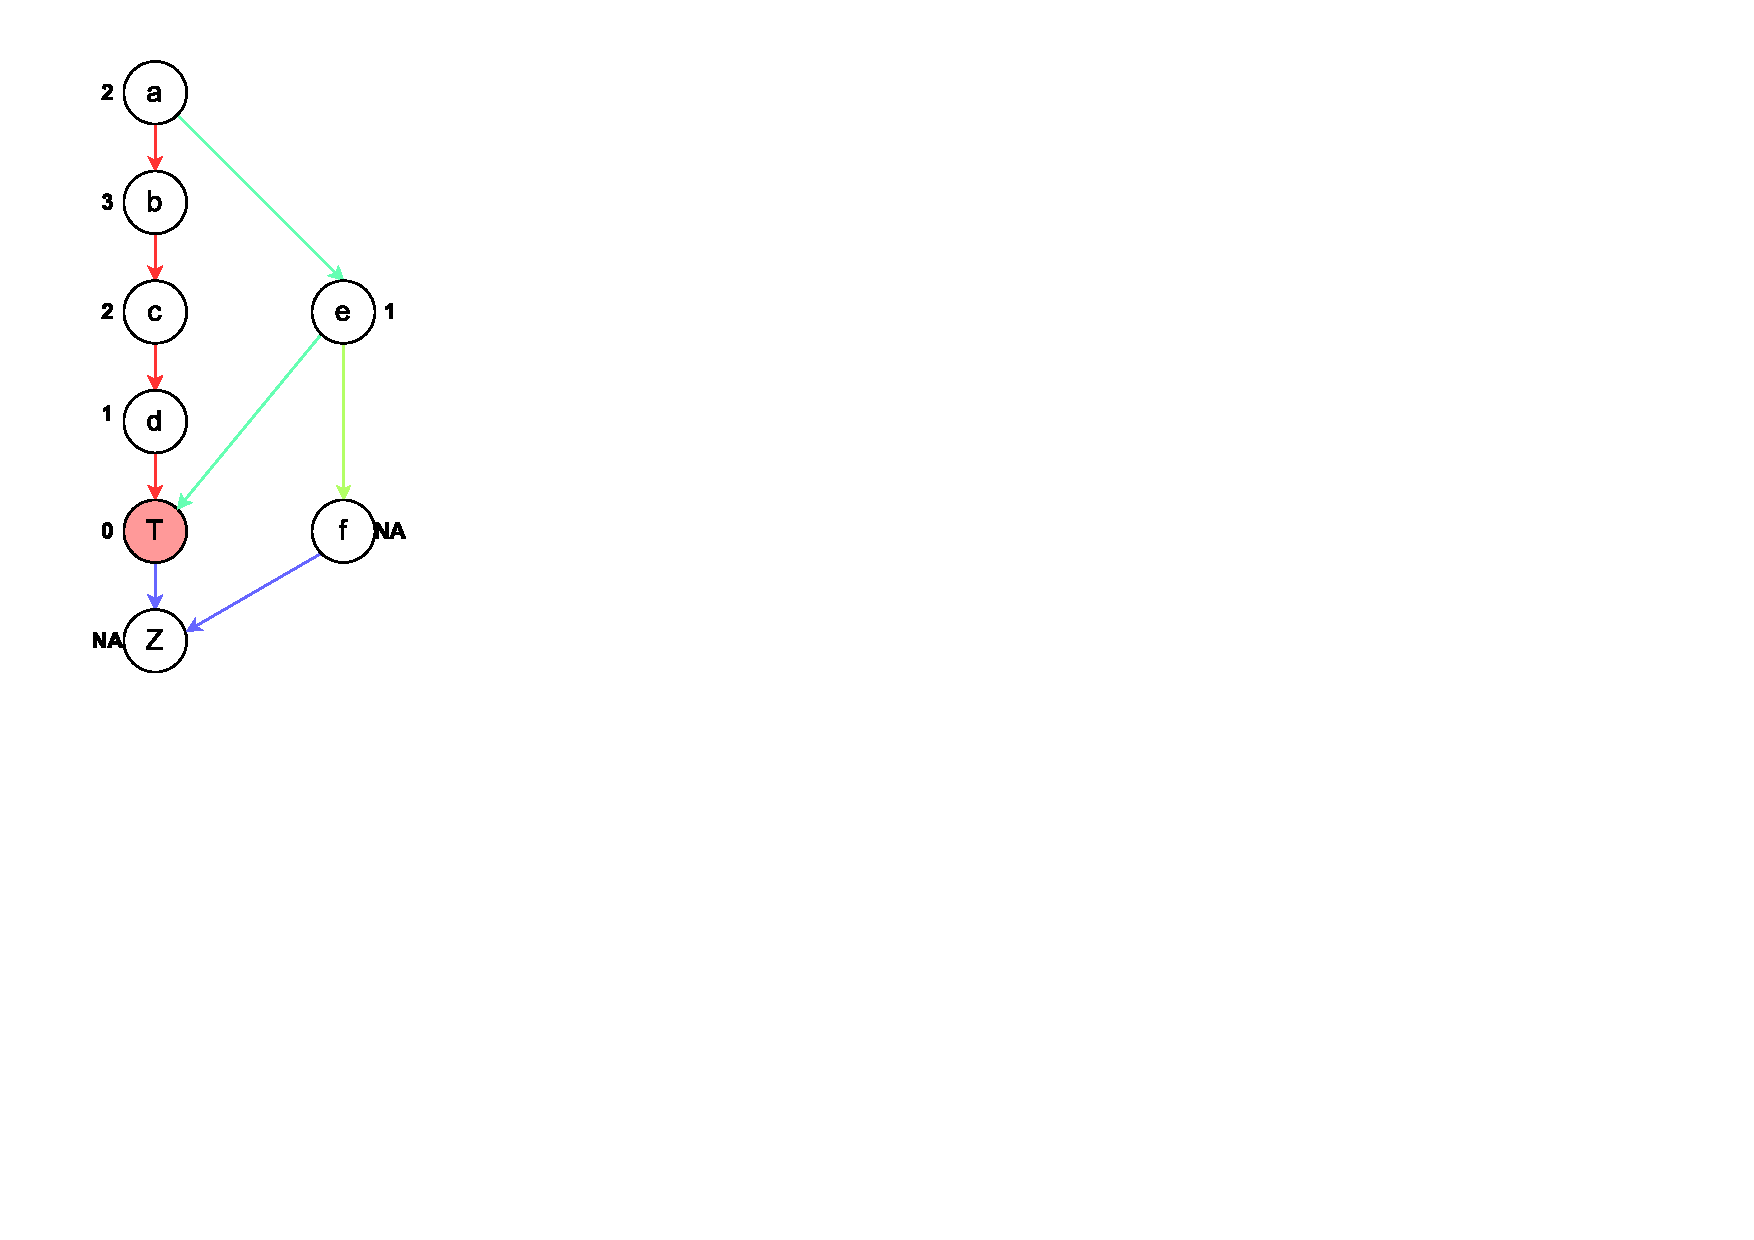
\includegraphics[width=0.3\textwidth]{trace.pdf}
	\caption{种子路径示例}
 	\label{pic:trace}
\end{figure}

让我们再重新审视种子目标距离的定义,即式\ref{eq:sdis}。其采取的计算方式是种子路径经过的基本块的基本块级目标距离总和除以
经过的基本块数。注意,由于轻量化插桩实现的机制,在实际计算过程中,种子目标距离计算时除以的是种子路径上经过的基本块级目标距离大于等于0的
基本块总数。

在图\ref{pic:trace}中提供了这样的一个例子。这是程序的部分调用图CG。为了简单起见,将每个函数中的基本块假设为1,那么我们就用函数级的
目标距离来代替基本块级目标距离来计算种子的目标距离。如图所示,假设$T$为目标函数,其余每个函数的目标距离已计算得出并在图中标出,
其中“NA”为不可达目标函数。假设三个种子的执行路径分别如下:
\begin{itemize}
	\item 种子S1:$a \to b \to c \to d \to T \to Z$
	\item 种子S2:$a \to e \to T \to Z$
	\item 种子S3:$a \to e \to f \to Z$
\end{itemize}
那么依据式\ref{eq:sdis},可以分别计算出种子目标距离$d(S1,T)=\frac{2+3+2+1+0}{5}=1.6$,$d(S2,T)=\frac{2+1+0}{3}=1$,
$d(S3,T)=\frac{2+1}{2}=1.5$。

按照DGF关于距离的定义机制是公平且不带有偏见性的原则,我们显然可以看出AFLGo设计的种子目标距离是具有一定的偏见性的:即AFLGo更倾向于
选择路径更短的种子。我们可以看到,能够到达目标函数的长路径种子S1的距离甚至比不能到达目标函数的短路径种子S3要远!这也意味着,如果实际
漏洞存在于较长的执行路径的话,AFLGo的偏向性会使得其花费更多的时间资源来探查到此漏洞。这显然与DGF的目标不符,也与设计原则冲突。究其原因,
是AFLGo采取了最短路径算法的距离定义和能量调度策略使得AFLGo倾向于更快地到达目标,而不是尽可能的覆盖测试所有可能到达目标的路径。

于是我们可以补充定义一个可达目标函数集覆盖率的指标来引导种子尽可能覆盖更多可能到达目标的路径。首先我们引入可达目标函数集$\zeta(T_f)$的概念,
$\zeta(T_f)$是被测试程序中所有可以到达目标函数集$T_f$中任一函数$t_f$的函数集。

\begin{algorithm}[H]
	\SetKwSty{algokeywordsty}
	\SetFuncSty{algofuncsty}
	\SetDataSty{algodatasty}
	\SetArgSty{algoargsty}
	\SetCommentSty{algocmtsty}
	\SetKw{break}{break}
	\SetKw{continue}{continue}
	\SetKw{not}{not}
	\SetKwFunction{dequeue}{\textsc{Dequeue}}
	\SetKwFunction{enqueue}{\textsc{Enqueue}}
	\SetKwFunction{isempty}{\textsc{IsEmpty}}
	\SetKwFunction{iscall}{\textsc{IsCall}}	
	\SetKwFunction{getProgram}{getProgram}
	\SetKwData{queue}{$\textit{Queue}$}
	\SetKwData{func}{$\textit{Function}$}
	\SetKwData{i}{$\textit{func}$}	
	\SetKwData{cg}{$\textit{CallGraph}$}	
	\KwIn{\targets\tcp{a finite set of targets}}
	\KwOut{\reach \tcp{a finite set of target-reachable functions}}
	$\reach \gets \varnothing$\;
	$\queue \gets \targets$ \; 
	\While {$ !\isempty(\queue) $}{
	  $\func \gets \dequeue(\queue) $\; 
	  \For{$\i \in \cg $}
	   {    
		\If{\iscall(\i,\func)}
		{
			\tcp{to be unique}
			\lIf{\i $\in$ \queue}{\continue}
			\enqueue(\queue,\i) \; 	
			$\reach \gets \reach \cup \i$\;	
		}
	   }
	}
	\Return{\reach}\;
	\caption[short]{计算可达目标函数集的不动点算法}\label{alg:point} 
\end{algorithm} 
\vspace{6pt}
算法\ref{alg:point}展示了一个简单的依据调用图CG计算$\zeta(T_f)$的不动点算法。利用此算法我们可以计算得到可达目标函数集,
由此可以定义种子的可达目标函数集覆盖率:
\begin{equation}
	C_s(s)=\frac{|\xi(s) \cap \zeta(T_f)|}{|\zeta(T_f)|}
\end{equation}
由此我们就得到了可达目标函数集覆盖率。不过由于在实际测试中,$\zeta(T_f)$一般为固定大小,故我们实际采用可达目标函数集覆盖量
$r(s)=|\xi(s) \cap \zeta(T_f)|$来做衡量即可。

在引入可达目标函数集覆盖量这一指标后,我们通过对其进行归一化处理得到$\widetilde{r}(s)$,将其引入能量调度公式(即式\ref{eq:energy}),
得到更新后的能量调度公式:
\begin{equation}
	p(s)=\widetilde{r}(s) \cdot (1-\widetilde{d}(s,T_b))\cdot(1-T)+0.5T
\end{equation}

\section{本章小结}
本章详细介绍了本文重点研究的灰盒模糊测试工具AFLGo及其框架结构。通过距离计算机制和能量调度机制详细分析了AFLGo实现
对被测试程序的定向策略。而后,本章结合示例指出其设计机制上的不合理之处,并针对性的进行了定向指标的补充设计和修改,包括
距离的重新定义和可达函数集覆盖率的设计。

\chapter{基于AFLGo的定向模糊测试系统的实现}
\section{需求分析}
软件测试是软件开发生命周期中非常重要的一环。在软件发布前和软件发布后维护都要大量的用到软件测试技术。
在软件发布前,开发人员通常会利用静态分析技术来查验软件中的错误。这种技术一般通过控制流分析、符号执行等方式进行测试,
以发现潜在的缺陷和漏洞。然而,由于静态分析技术是在不对程序实际运行的情况下进行分析,因此难免会出现大量的误报。在以往的测试过程中,
往往需要投入使用大量的人力资源来进行分析测试,以便尽可能地排除这些误报。但是,这样做的成本非常高昂,并且效率低下。
定向模糊测试能够基于静态分析提供的定位信息,针对具体的代码段生成有效的测试用例,从而验证静态分析结果的正确性。
通过结合静态分析和定向模糊测试,可以大幅度减少人工测试的工作量,并提高测试效率和准确性。这种方法不仅可以帮助开发人员更加迅速
和准确地发现程序中的潜在问题,同时还能够提升软件的质量和可靠性,更好地保障软件的安全性和稳定性。

在软件的维护期间,为确保已发布的软件版本或修复了某些漏洞的安全补丁能够有效、可靠和稳定地运行,需要进行细致的补丁测试工作。
这项工作通常包括多个方面的测试,例如功能测试、性能测试以及安全测试等。其中,针对已发布的软件版本或修复了某些漏洞的安全补丁
进行的验证测试非常重要。这些测试可以帮助开发团队确定所发布的软件版本或安全补丁是否真正解决了之前存在的漏洞或问题,并且能够
在不引入新漏洞的情况下提供稳定的功能。除了验证测试外,采用定向模糊测试也是一种有效的方式。通过引入针对修补部分的位置信息,
定向模糊测试可以自动化地检测补丁是否正确地修复了漏洞,同时也能够检测新的漏洞是否被引入到系统中。

在第三章中,我们介绍了定向的重要性,并给出了两项针对AFLGo定向策略的改进方法。通过这种改进,AFLGo可以更加全面地实
现定向模糊测试,从而提高测试效率和发现漏洞的概率。本文采用了第三章提出的策略设计,并对AFLGo进行了修改和集成。通过
这些修改和集成,可以使AFLGo能够更加高效地执行定向模糊测试,并且可以应对包括上述两种应用场景在内的仅包含目标代码区域的
定向覆盖测试任务。这些改进使得AFLGo成为一个更加强大和灵活的测试工具,可以帮助开发人员更好地发现和修复软件漏洞。

\section{距离机制的改进实现}
如\ref{sec:AFLGo}节中所言,AFLGo的预处理部分包含两次编译处理来计算距离和实现插桩。其中第一次编译处理和第二次编译处理实际上都
是利用了同一个LLVM的pass插件\cite{Pass}实现的,具体流程可参考图\ref{pic:pass}。为了延续图\ref{pic:AFLGo}中AFLGo的架构介绍,
针对此pass插件的具体修改将分别对应框架结构中不同部分的修改来相应介绍。

\subsection{图生成器的改进}
AFLGo预处理阶段所依赖的每个函数对应的CFG都是在pass插件的第一次编译过程中生成的。事实上一些比较重要的信息,例如所有基本块的标识,
所有函数的函数名,以及函数间的调用关系等都是在此阶段生成。此过程的实现过程是利用Clang\cite{Clang}将源码转换为LLVM的中间表示
(Intermediate Representation,简称IR),而后通过针对IR执行相应的操作从而实现控制流图的生成,函数调用图的生成等静态分析部分。

在这一部分,在利用Pass进行基本块级的遍历分析时,还将额外记录基本块及其所在函数以及所调用函数的信息。
利用这一原始信息,我们就可以计算得到每个函数中对应的因子函数(式\ref{eq:factor1},式\ref{eq:factor2}计算得到)。这将为后面
计算函数级距离提供基础。

\begin{figure}[htb]
	\centering
	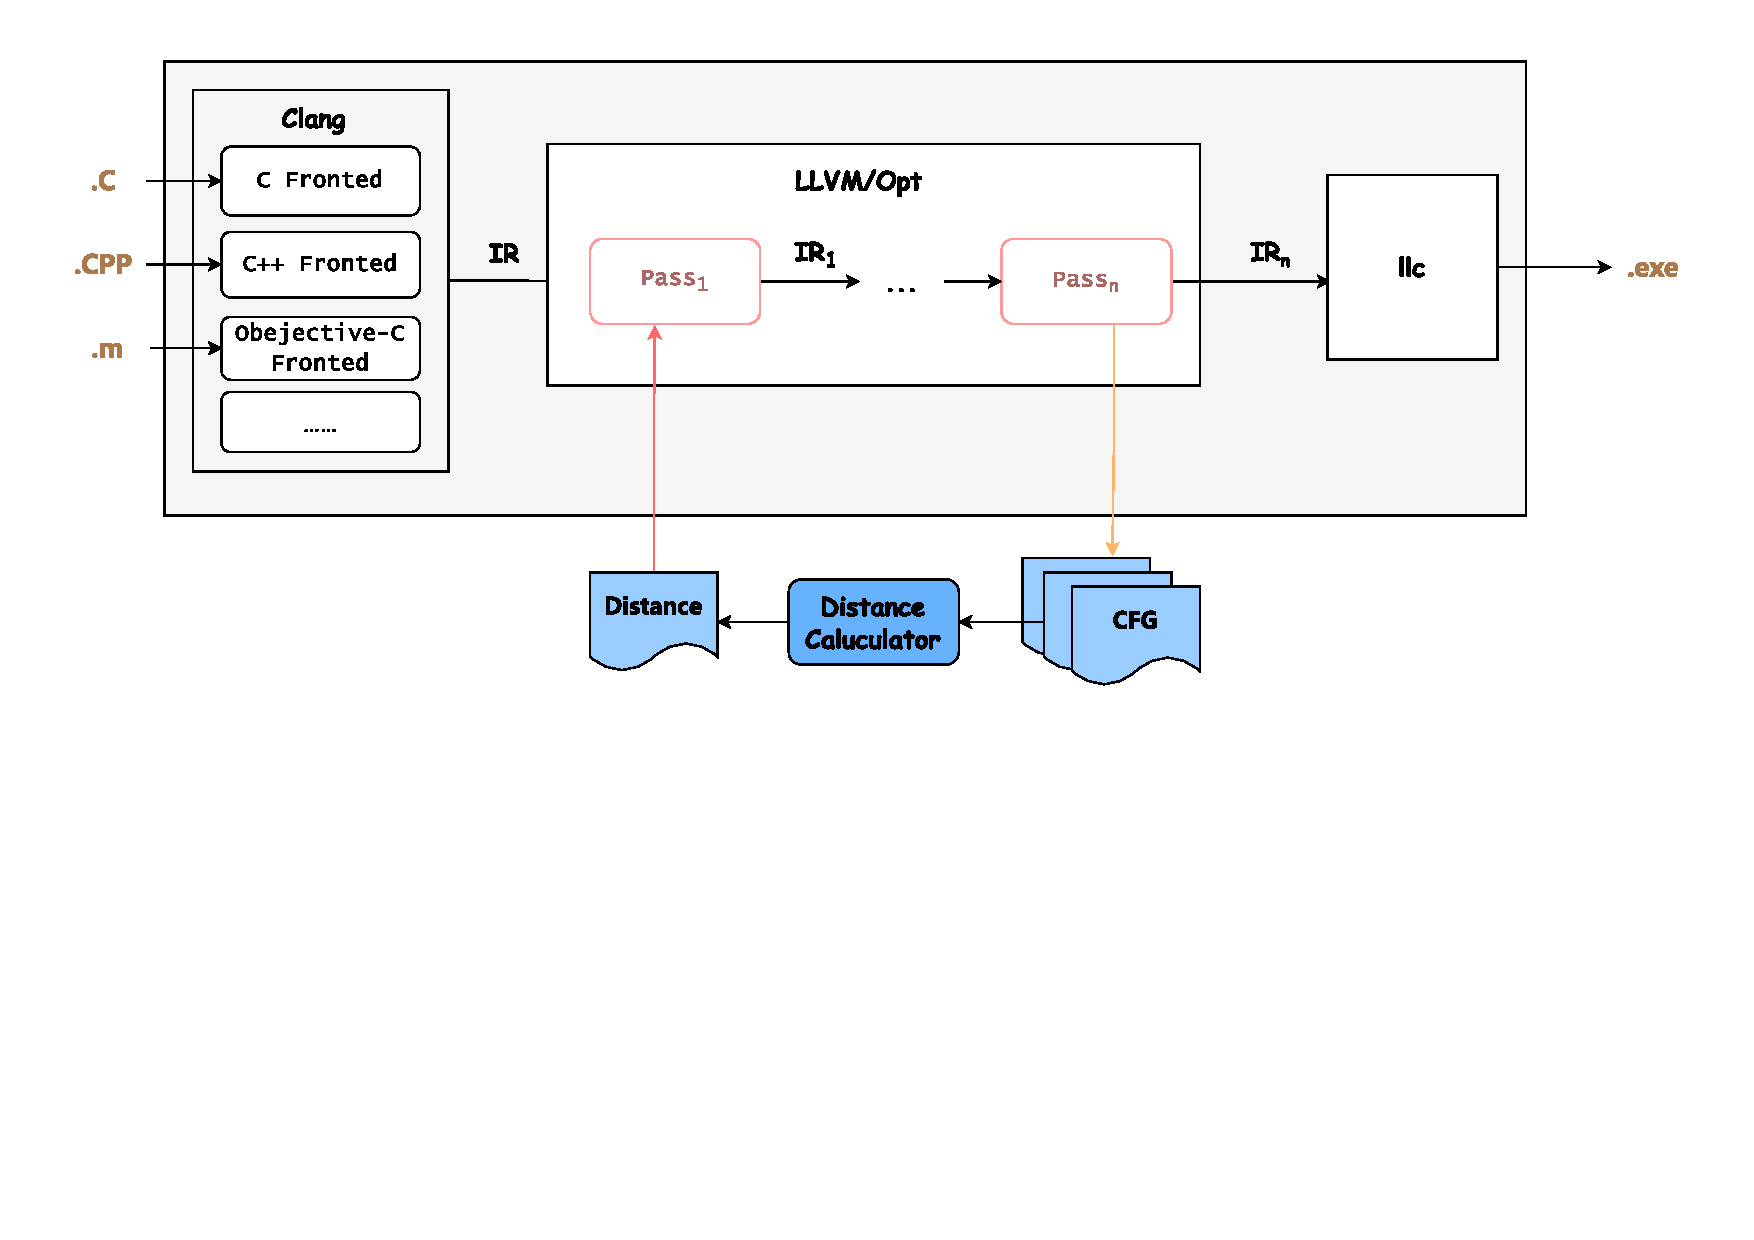
\includegraphics[width=1\textwidth]{pass.pdf}
	\caption{LLVM以及Pass插件的工作实现}
 	\label{pic:pass}
\end{figure}


\subsection{距离计算器的改进}
在得到每个函数及其对应的因子后,在距离计算器中将重构调用图生成部分。
AFLGo会将图生成器生成的调用图CG输入距离计算器中,而后利用C++中的经典库Boost\cite{Boost}来将计算目标距离转换为图
的求最短路径问题。由于AFLGo采用的是一个无权图的结构,直接结合广度有限搜索(BFS)算法即可计算得到函数级距离。

利用已得到的因子结合式\ref{eq:ffdis}即可计算得到的调用函数间相邻的距离。这一重新定义的距离也为CG引入了权重。
于是在距离计算器中调用图将重新建模为有权图,这时就要引入迪杰斯特拉最短路径算法用以计算函数级的目标距离。
至此,AFLGo距离机制就完全被修改完成了。

除了在对距离计算器做了如此改进以外,还额外实现了利用调用图按照算法\ref{alg:point}计算可达目标函数集的步骤。这一步将为
后续的可达目标函数集覆盖量的计算提供基础。

\section{可达目标函数集覆盖量的计算实现}
\subsection{AFLGo插桩器的原理}
在介绍对可达目标函数集覆盖量的计算实现前我们需要先了解AFLGo的插桩器原理。

AFLGo的插桩器是基于AFL框架的LLVM mode实现的。作为LLVM的编译前端,Clang将在编译时将被测试程序的源码转换为LLVM IR。结合Pass,
Clang可以在编译为源码为IR后遍历每个函数的每个基本块,然后Pass会随机生成一个int型数据分配给当前基本块作为标识。而后会将当前基本块
的表示与前一个经过的基本块的int型标识异或作为从前一基本块至当前基本块的路径的标识,最终,AFL会将此路径标识转换为运行时的共享内存块
的偏移地址,从而实现从共享内存块中收集到一次实际的程序执行执行过的路径信息。这一步也就实现了AFL编译器级的插桩效果。

AFLGo在此基础上做出了基于其自己的修改。由距离计算器得到的每个基本块的基本块级目标距离将在Clang编译伊始作为辅助信息送入。而后在编译时,
根据每个基本块的基本块级目标距离是否大于等于0来判断决定此基本块处是否要额外插桩执行代码。AFLGo在AFL申请的共享内存基础上额外申请了16字节的
空间,用以记录两个运行时变量:经过的总距离(8字节)和经过的总基本块数(8字节)。如果Pass遍历过程中依据距离信息判断此处应该插入执行代码,
那么其就会在此基本块处额外插入执行以下步骤的代码:
\begin{enumerate}[label=(\arabic*)]
	\item 将共享内存块M中存储总距离变量的内存地址M[a]处的数值$d_1$取出
	\item 将当前基本块对应的基本块级距离$d_2$与$d_1$相加得到更新后的$d_1^\prime$
	\item 将$d_1^\prime$存回M[a]
	\item 将M中存储经过的总基本块数量的内存地址M[b]处的数值$c_1$取出
	\item 将$c_1$加一得到更新后的$c_1^\prime$ 
	\item 将$c_1^\prime$存回M[b] 
\end{enumerate}

上述代码在编译期间插桩后,在被测试程序执行时运行到相应的基本块位置会直接执行。这样,在将种子执行完成后AFLGo的控制器部分将可以依据
共享内存中收集得到的信息得到种子此次执行的总距离和经过的总基本块数,就可以用以计算得到种子的目标距离。这就为后续的能量计算和调度提供了
关键信息。
\subsection{插桩器的修改}
\begin{figure}[htb]
	\subfigure[路径示例]{
		\begin{minipage}[b]{0.5\textwidth}
			\centering
			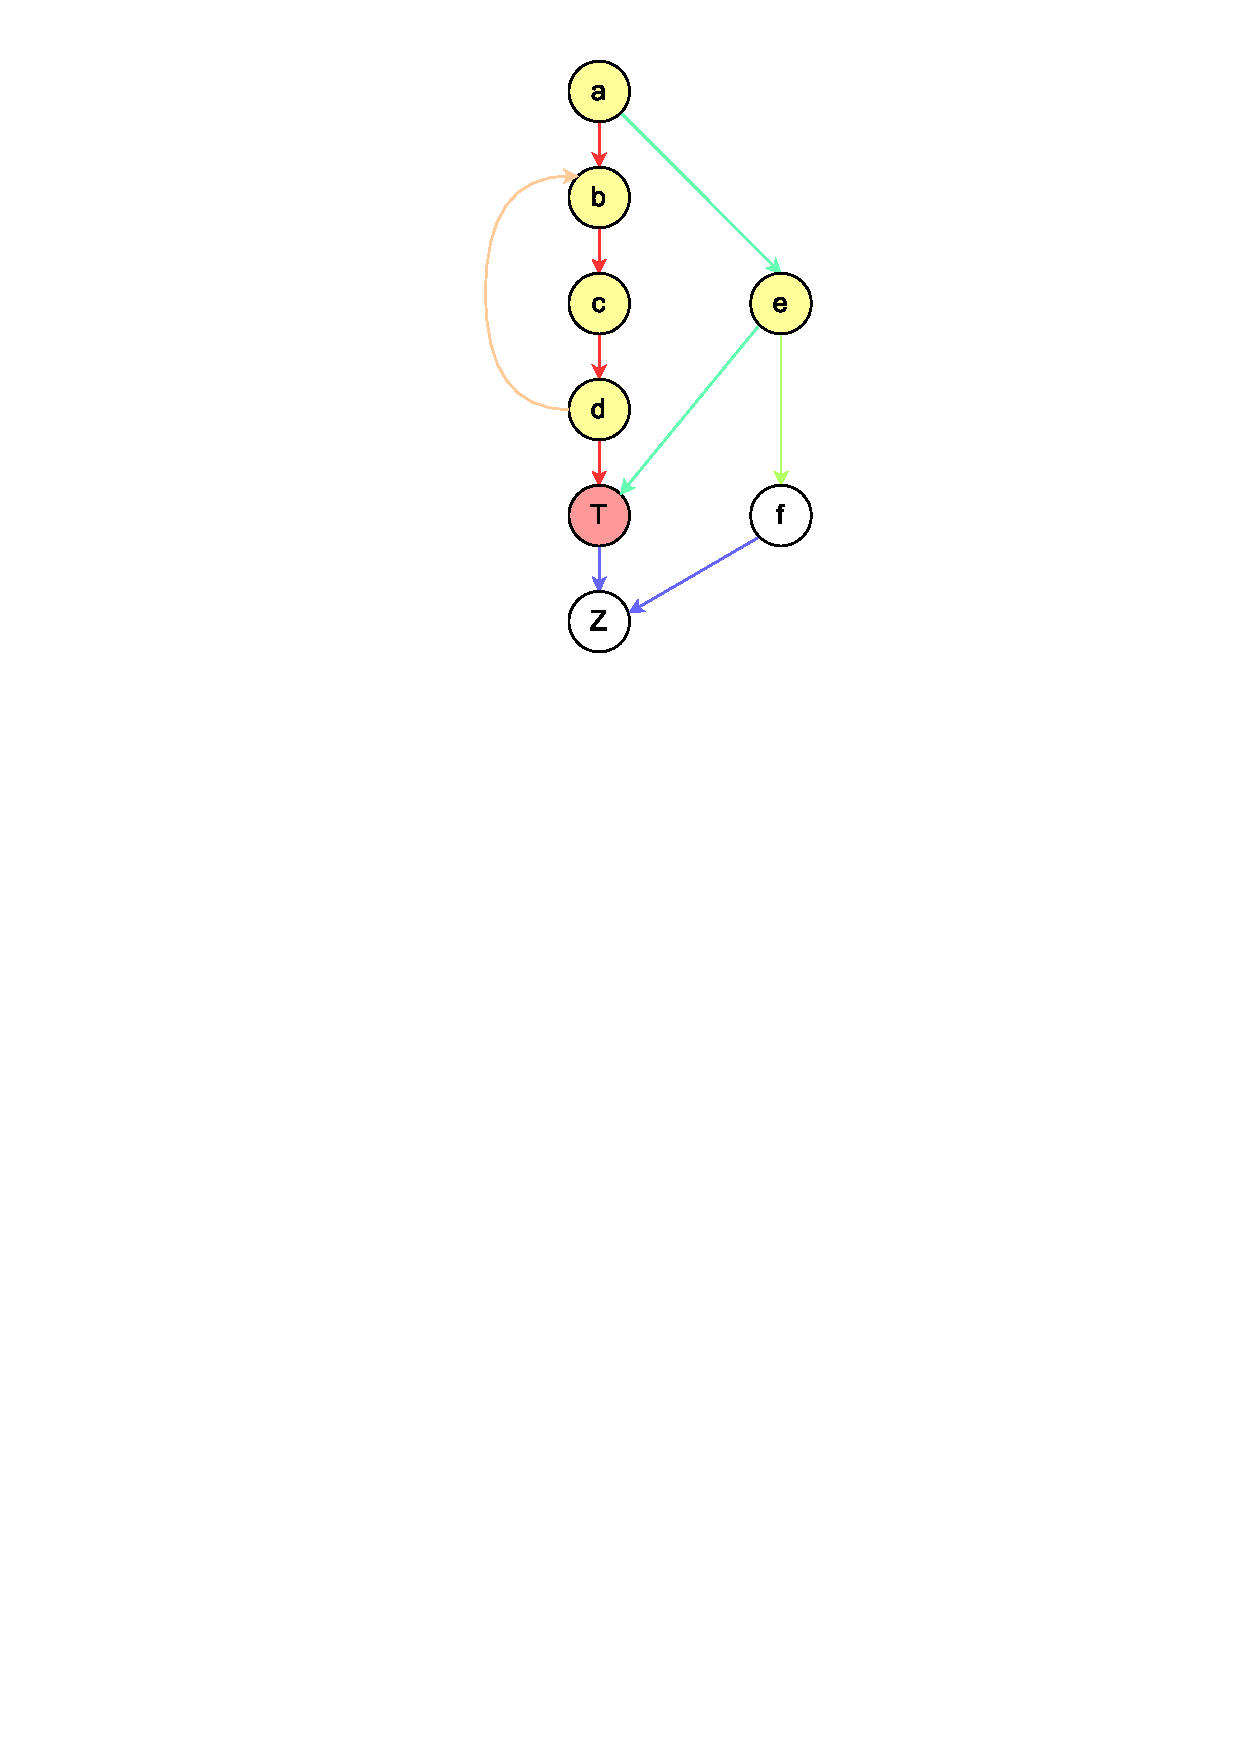
\includegraphics[width=0.5\textwidth]{fc1.pdf}
		\end{minipage}
		}\\
	\subfigure[共享内存]{
		\begin{minipage}[b]{0.95\textwidth}
		 	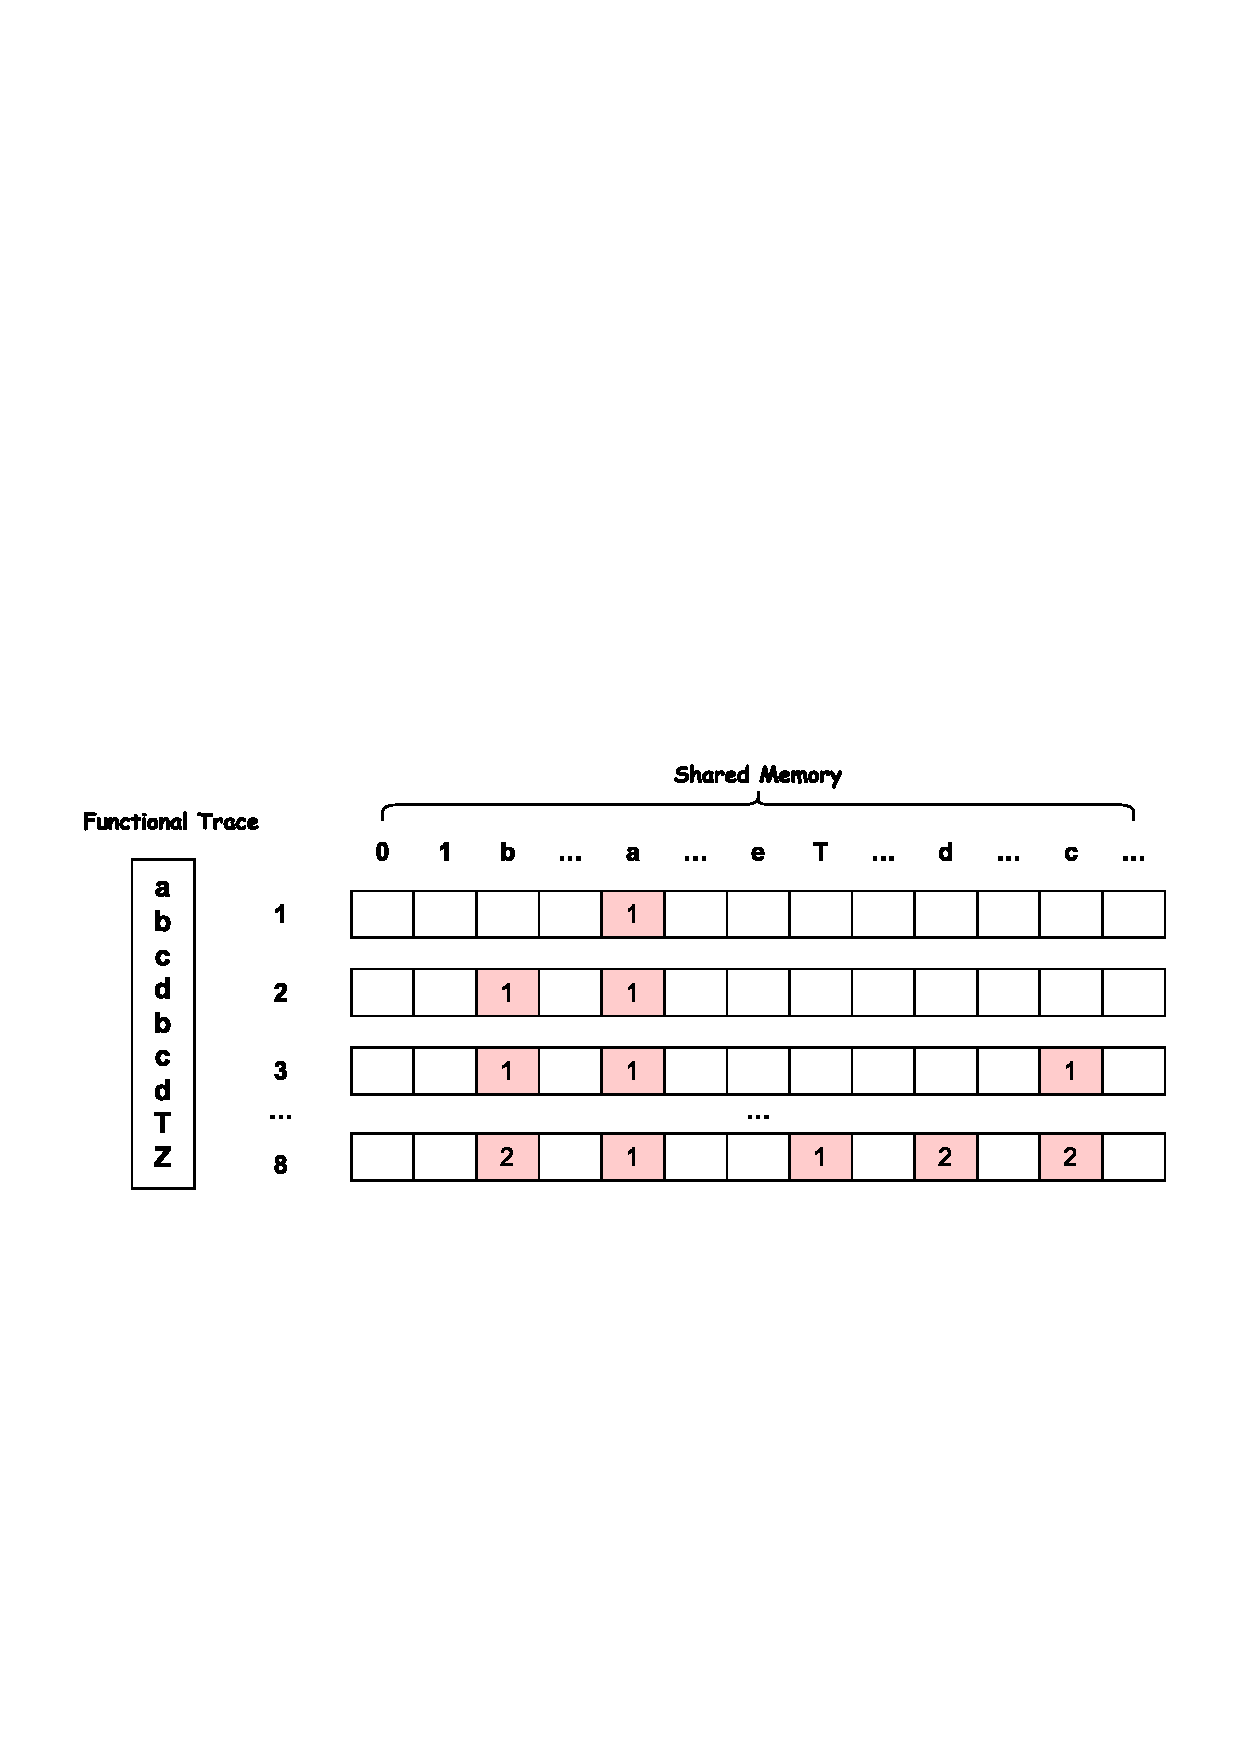
\includegraphics[width=1\textwidth]{fc2.pdf}
		\end{minipage}
		} 
	\caption{可达目标函数集计算示例}
 	\label{pic:fc}
\end{figure}

本文实现的针对于插桩器的修改是在AFLGo申请的共享内存空间大小上再此额外申请16kB。这部分内存将用于记录被测试程序经过的已被覆盖的
可达目标函数集的函数。

这块内存将被视作一个大数组,数组中的元素占一个字节。同AFL标识基本块的原理相同,在本文的实现中,会将每一个函数的第一个基本块表示为
函数的代表。通过给此基本块赋[1,16K]间的随机值来标识函数。当在Pass的执行过程中识别到当前被遍历到的函数处于可达目标函数集中,就会
为其额外插桩一段执行代码:

\begin{enumerate}[label=(\arabic*)]
	\item 获得当前函数被赋予的随机值r
	\item 将共享内存中M中对应的M[r]位置处的数值$c$取出
	\item 将$c$加一得到更新后的$c^\prime$
	\item 将$c^\prime$存回M[r] 
\end{enumerate}

这段代码的执行逻辑与AFL的执行逻辑相同。通过执行这一步骤,我们就可以获取被测试程序在运行完种子后,种子路径所覆盖的可达目标函数集中的函数
量。

图\ref{pic:fc}展示了一个简单的示例。其中(a)图为调用图示例,以图\ref{pic:trace}为基础,为了贴合实际,加上了
环路来展现实际可能的函数调用链。(b)图展现了一个种子可能的路径$a\to b \to c \to d \to b \to c \to d \to T \to Z$。
由可达目标函数集的定义我们可以知道$\xi(T)=\{a,b,c,d,e,T\}$。经过插桩以后,当被测试程序执行此种子时,共享内存的
情况就如图(b)所示。最后,通过分析共享内存中不为0的内存块数,就可以得知此种子覆盖的可达目标函数为$\{a,b,c,d,T\}$,
数量为5。在计算得到此值后,就可以通过参与能量调度实现定向。

当然,这一方法可能存在着一些问题。事实上,这一段共享内存的使用本质上是一个哈希表。我们难以保证随机给不同的函数的随机值会一定不同。
但是,实际可达目标函数的函数集数量并不会很大。以libxm2为例,整个项目的文件共有3235个函数,若设定目标函数为“xmlAddID”,那么其对应的
可达目标函数集的大小仅为344。考虑到设定随机数的取值范围为16k,这使得标识相撞的可能性较低。
此外,相比于额外确定计算可达目标函数在整体程序中的调用分布和一一对应到共享内存的标识所付出的额外的时间,
少数的标识相撞所带来的导引精度损失是更加可接受的。

\section{本章小结}
本章结合定向模糊测试的需求分析,详细介绍了基于第三章提出的针对于AFLGo的两项改进机制的具体实现方式。详细介绍了针对于AFLGo中
插桩器和距离计算器部分的修改,结合示例展示了实现方式。

\chapter{系统测试}
\section{系统测试概述}
\subsection{系统测试环境}
本文的系统测试及评估运行在个人笔记本电脑中。其中处理器配置为英特尔 Core i5-8265U 四核处理器,标准主频为1.60GHz,
内存大小为16GB,操作系统为WSL2-Ubuntu 20.04(64位)。

\subsection{系统测试目标}
本文执行的系统测试主要目标包括以下几部分:
\begin{enumerate}[label=(\arabic*)]
	\item 验证本文设计实现的机制在AFLGo架构下插入的正确性和有效性。将通过实际执行系统功能测试和输出结果,验证机制被正确集成进入框架。
	通过执行实际的测试项目,验证机制植入的有效性;
	\item 验证实现的定向灰盒模糊测试工具的性能:将通过测试本文实现的定向灰盒模糊测试工具(下称AFLGo$^\prime$)实际的系统功能,考察其作为定向灰盒模糊测试
	工具针对特定代码区域导致的错误或脆弱性缺陷的检出率。这部分将与AFLGo和AFL++\cite{aflpp}进行比较。此外,还将分析比较在实际程序中执行测试
	的性能差异。
\end{enumerate}

\section{功能测试}
\subsection{距离机制集成的有效性}
本小节将对本文实现的AFLGo$^\prime$中距离机制集成的有效性进行验证。

\begin{table}[hbp]
	\centering
	\begin{tabular}{|c|c|c|c|c|c|}
	  \hline
	  项目 & 被测试程序 & 总函数量  &函数间调用 &$C_B >1$ & $C_N >1$ \\
	  \hline
	  GNOME & libxml2 & 3235 &9973  & 3027 &  2839\\
	  \hline
	  Binutils & cxxfilt & 5184 & 13524  & 4339 & 3945\\
	  \hline
	  mjs & mjs & 385 & 1200  &  325 & 271\\
	  \hline
	  Binutils & objdump & 5301 & 14057 &  4558 &  4155\\
	  \hline  
	\end{tabular}
	\caption{被测试程序静态分析数据}\label{tab:sa}
  \end{table}
表\ref{tab:sa}是主要针对于主要被测试程序的静态分析数据。选取的被测试程序包括libxm2\cite{Libxml2},cxxfilt\cite{cxxfilt},mjs\cite{mjs}
以及objdump\cite{objdump}。主要针对被测试程序做了函数级的静态分析。表中总函数量表明统计得到的程序中总包含的函数数量。函数间调用则是
通过分析得到的函数间调用关系总量,后两项则记录的是在章节\ref{sec:disredefine}中额外补充定义的函数间调用两个影响因子大于1的函数量。
可以看到,后两项$C_B >1$和 $C_N >1$的函数占比在总项目中的比例都很大,这从实际上证明了考虑函数间不同模式的调用关系的重要性。

下面的主要以libxm2作为被测试程序为例说明距离机制集成的有效性。
为了与参考实验论文做对比,本文主要选择使用了libxml2 20904-GITv2.9.4-16-g0741801的历史版本来对比测试。
如无特殊说明,后文中的libxm2均指本版本。在本小节,将主要与AFLGo对比距离机制是否有效集成进入本文实现的模糊测试工具。

代码\ref{code:target}给出了本次实验中的libxm2的目标区域,其中前面表明代码所在文件,后面数字表示目标代码所在的代码行。
该部分代码是libxm2开发者在修复已知的错误时经由ef709ce2提交的补丁版本。
其对应的所在的目标函数为xmlAddID。为了验证修改的距离机制是有效的,代码\ref{code:callsite}展示了被测试程序中部分函数的函数级目标距离,
其中前面表示函数名,后面的数字表示函数级目标距离。其中,old distance注释下的部分是指在旧的AFLGo距离机制下计算得到的函数级目标距离,
而new distance注释下的部分是指在新的距离计算机制下计算得到的函数级目标距离。

\renewcommand{\thelstlisting}{5.\arabic{lstlisting}}
\begin{lstlisting}[caption={指定目标代码区域行号},label={code:target}]
	valid.c:2637
	valid.c:2638
	valid.c:2639
	valid.c:2640
\end{lstlisting}

可以看到,在旧的AFLGo默认距离算法下相同函数级目标距离的函数streamFile和testSAX,xmlParseNotationDecl和xmlParsePI在新的
距离算法下被做出了不同调用模式的区分。考虑到事实上的AFLGo的函数级目标距离的实际意义是当前函数沿着调用链至目标函数的最少调用次数
,在集成距离机制后的新距离算法下可以看见经过相同调用次数的函数级目标距离依然在数值上保持接近,可以认为新的距离机制
机制被正确地集成进入AFLGo$^\prime$中。

\renewcommand{\thelstlisting}{5.\arabic{lstlisting}}
\begin{lstlisting}[caption={先后目标距离对比},label={code:callsite},basicstyle=\linespread{0.85}\ttfamily\small]
	//old distance
	main,6
	streamFile,9
	testSAX,9
	xmlParseNotationDecl,14
	xmlParsePI,14
	...

	//new distance
	main,10.673611111111111
	streamFile,16.25
	testSAX,17.625
	xmlParseNotationDecl,28.875	
	xmlParsePI,27.890625000000004	
	...
\end{lstlisting}
\subsection{定向覆盖的有效性}
本小节将验证AFLGo$^\prime$的定向覆盖测试的有效性。

\begin{table}[htbp]
	\centering
	\begin{tabular}{|c|c|c|c|c|c|}
	  \hline
	  测试次数 & 测试时长(s)& TTE(s)&总执行路径& 检出崩溃次数 &目标区域引起 \\
	  \hline
	  1 & 8166 & 609 & 2767  &30 & 30\\
	  \hline
	  2 & 9409 & 360 & 2894  &16& 16\\
	  \hline
	  3 & 6322 & 524 & 3034  & 16& 16\\
	  \hline
	  4 & 8401 & 918 & 3166 &  23 & 23\\
	  \hline 
	  5 & 5088 & 1000 & 2551&  12 & 12\\
	  \hline  
	\end{tabular}
	\caption{AFLGo$^\prime$的模糊测试情况}\label{tab:aflgop}
\end{table}

由于很难给出有效的定向覆盖测试的评估指标,在本小节将采用由目标代码区域引起的漏洞或脆弱性的暴露情况来参与评估。本测试的
被测试程序依然同上一小节,主要以针对libxm2的分析为例,判断AFLGo$^\prime$的定向覆盖的情况。

由于模糊测试具有随机性,故而需要多次测试取均值来评估一般情况。表\ref{tab:aflgop}展示了其中的5次测试数据。多次测试均
采用设定45分钟为探索-开发阶段的分界时间。其中TTE(time-to-exposure)为第一次漏洞暴露时间;总执行路径是模糊测试此轮
测试中检出的总共的不同的执行路径;检出崩溃次数是模糊测试工具测出的独特崩溃(unique crashes)次数,而不是崩溃总次数。

可以看出,在相近的时间限制范围内,AFLGo$^\prime$检出的独特崩溃次数基本相近,总执行路径也基本相近。考虑到由于随机过程导致的差异性,
可以认为AFLGo$^\prime$的漏洞检出能力较为稳定。关于由目标程序引起,这指的是检出的崩溃中可以被确定是由目标区域引起的崩溃。

在本次测试中,对于libxml2本文采用了CVE-2017-\{9047,9048\}作为检测AFLGo$^\prime$定向覆盖有效性的指标。CVE-2017-9047\cite{47CVE},
CVE-2017-9048\cite{48CVE}是由libxml2在ef709ce2提交直接引入的错误。开发人员通过向valid.c中的方法xmlAddID函数
添加边界检查来修补空指针取消引用,也即代码\ref{code:target}中的行数位置。此函数由另外两个函数xmlParseOneAttribute
和xmlValidateOneNamespace调用。为了到达这些函数,解析器必须首先执行xmlValidateOneElement。当这个函数在函数的
不同点打印元素的内容时,这两个错误就会暴露出来。

在valid.c中的函数xmlSnprintfElementContent应该递归地将元素内容定义转储到大小为“size”的字符缓冲区“buf”中。
变量len被赋值为strlen(buf)。如果content->type是XML\_ELEMENT\_CONTENT\_ELEMENT,则将content->prefix附加到buf中,
然后将content->name写入缓冲区。然而,检查content->name是否适合也使用'len'的值而不是已更新的缓冲区长度strlen(buf)。
这使我们能够写入超过分配内存的“size”个字节,从而在实际测试中就会表现为内存溢出。

\renewcommand{\thelstlisting}{5.\arabic{lstlisting}}
\begin{lstlisting}[caption={示例错误打印栈},label={code:stack},basicstyle=\linespread{1.75}\fontsize{6.8}{5}\ttfamily]
Program received signal SIGSEGV, Segmentation fault.
#0  0x578447 in xmlDumpElementContent (buf=0x934c00, content=0x93f3f0, glob=1) at valid.c:1175
#1  0x578125 in xmlDumpElementDecl (buf=0x934c00, elem=0x942710) at valid.c:1706
#2  0x8a4c3a in xmlBufDumpElementDecl (buf=0x934e90, elem=0x942710) at xmlsave.c:501
#3  0x8a8943 in xmlNodeDumpOutputInternal (ctxt=0x9427f0, cur=0x942710) at xmlsave.c:939
#4  0x8b57f1 in xmlNodeListDumpOutput (ctxt=0x9427f0, cur=0x942710) at xmlsave.c:825
#5  0x8b5250 in xmlDtdDumpOutput (ctxt=0x9427f0, dtd=0x93f300) at xmlsave.c:749
#6  0x8a87f8 in xmlNodeDumpOutputInternal (ctxt=0x9427f0, cur=0x93f300) at xmlsave.c:931
#7  0x8a7dcc in xmlDocContentDumpOutput (ctxt=0x9427f0, cur=0x93f220) at xmlsave.c:1234
#8  0x8a635c in xmlSaveDoc (ctxt=0x9427f0, doc=0x93f220) at xmlsave.c:1936
#9  0x419833 in parseAndPrintFile (filename=0x7fffffffe412 "seed", rectxt=0x0) at xmllint.c:2705
#10 0x40cd0e in main (argc=5, argv=0x7fffffffe128) at xmllint.c:3759
\end{lstlisting}

代码\ref{code:stack}展示了一个崩溃示例的打印栈情况。可以看到,AFLGo$^\prime$生成的种子引起了xmlDumpElementContent的错误内存访问。
代码\ref{code:bug}是引起错误的部分代码片段。这部分的逻辑则是由于content->c1->type的类型为XML\_ELEMENT\_CONTENT\_SEQ,
则重复递归xmlDumpElementContent函数将元素内容定义转存至缓冲区。由此,可以确定这一崩溃漏洞是由目标区域引入导致的。

\renewcommand{\thelstlisting}{5.\arabic{lstlisting}}
\begin{lstlisting}[caption={示例错误函数},label={code:bug},numbers=left,firstnumber=1174,numbersep=-2em,numberstyle=\footnotesize ]
	case XML_ELEMENT_CONTENT_SEQ:
		if ((content->c1->type == XML_ELEMENT_CONTENT_OR) ||
			(content->c1->type == XML_ELEMENT_CONTENT_SEQ))
		xmlDumpElementContent(buf, content->c1, 1);
		else
		xmlDumpElementContent(buf, content->c1, 0);
			xmlBufferWriteChar(buf, " , ");
		if ((content->c2->type == XML_ELEMENT_CONTENT_OR) ||
			((content->c2->type == XML_ELEMENT_CONTENT_SEQ) &&
			(content->c2->ocur != XML_ELEMENT_CONTENT_ONCE)))
			xmlDumpElementContent(buf, content->c2, 1);
		else
			xmlDumpElementContent(buf, content->c2, 0);
			break;
\end{lstlisting}

在系统测试的统计结果中可以知道,AFLGo$^\prime$生成的测试用例确实触发了由目标区域引入导致的错误,我们可以认为本文实现的灰盒定向模糊测试
工具AFLGo$^\prime$具有良好的定向覆盖测试的特性。
\section{性能评估}
在本小节将使用本文集成实现的AFLGo$^\prime$与采取的集成测试工具AFLGo以及AFL的后续社区项目AFL++进行对比,从而尝试针对AFLGo$^\prime$
的性能进行评估。由于本文设计的指标是针对AFLGo定向策略中的偏见性做出修正而出发实现的,故而为了确认定向策略的修正
以及本文的采取的集成方式不会对模糊测试器的性能做出影响,采取与AFLGo和AFL++对比评估AFLGo$^\prime$的性能。

\begin{table}[htbp]
	\centering
	\begin{tabular}{|c|c|c|c|c|}
	  \hline
	  测试工具 & TTE(s)&执行路径元组& 检出错误类型 &目标区域引起 \\
	  \hline
	  AFLGo$^\prime$ & 607 & 2882 & 2  & 100\% \\
	  \hline
	  AFLGo & 689 & 3032 & 4  & 26.7\%\\
	  \hline
	  AFL++ & 245 & 5176 & 4  & 44\%\\
	  \hline  
	\end{tabular}
	\caption{性能对比测试}\label{tab:aflgot}
\end{table}

表\ref{tab:aflgot}是上述三种模糊测试工具针对同一被测试程序在相同测试条件下进行模糊测试执行得到的结果对比。由于模糊测试的随机性,
上述数据均采用了多次实验取均值的方式。其中AFLGo和AFLGo$^\prime$均设置了相同的探测-开发阶段的分界时间。本实验使用的被测试程序依然是
libxml2,目标区域设置与前文相同。

由于AFLGo和基于AFLGo做出改进的AFLGo$^\prime$均是基于AFL2.52b版本做出的改进开发,而AFL++则是后续社区开发优化后的框架,故而由TTE指标中可以
看到AFL++检测出程序的第一个崩溃的平均用时更短。这与AFL++在种子变异策略等多方面对AFL进行了优化重构有关,当然也与AFLGo以及AFLGo$^\prime$在
种子生成调度上采取了定向策略有关。

执行路径元组总数可以在一定程度上衡量对于被测试程序的路径覆盖情况。元组(tuple)这一概念来源于AFL的路径识别方式。以图\ref{pic:trace}中的调用图
来做举例,由$a\to b$的一条调用边可以被视作一个元组,不过在AFL中这一概念是基本块级的。此外,$a \to b , b \to a$会被识别成两个不同的元组。简单来讲,
元组可以被视作基本块之间的路径。因而这一指标可以指示模糊测试工具对程序的覆盖率情况。可以看到,AFLGo$^\prime$,AFLGo,AFL++的执行路径元组是依次
增加的。这在一定程度上可以反应模糊测试工具的定向性是依次降低的。

在错误类型检出情况中,除了前文已经提到的CVE-2017-\{9047,9048\},还可以确定AFLGo与AFL++均探测到了CVE-2017-9049\cite{49CVE},CVE-2017-9048\cite{50CVE}。
这两个错误是由于对以前已经报告的错误CVE-2016-1839\cite{39CVE}的不完全修复导致的,AFLGo和AFL++依然产生了少量的测试用例可以触发此错误。由于这一错误并非
是由于目标区域的代码引入,所以在实验中并未将其作为复现目标。这部分的测试用例应当是由于AFL的灰盒模糊测试的基础框架生成,由于AFLGo$^\prime$的探测重点更集中于
可以到达目标区域的路径,这样的能量调度使得其并未生成探测到此错误。

目标区域引起的数据百分比则是由模糊测试工具报告的崩溃中可以确定是由CVE-2017-\{9047,9048\}导致的崩溃示例的占比。这也在一定程度上说明AFLGo$^\prime$
更加具有定向性。

综合上述实验结果的分析,我们可以得出结论:本文实现的AFLGo$^\prime$的定向模糊测试工具在定向测试目标上实现的更好,相比于AFLGo,本文实现的测试工具
将更多的精力放在了指定区域的路径探索。但是相应地,相比于AFL++,本文的AFLGo$^\prime$牺牲了一定的性能和对被测试程序的覆盖率扩张,导致可能会遗漏部分
非目标区域引进的错误;相比于AFLGo,AFLGo$^\prime$的性能的差距并不是很大,可以认为AFLGo$^\prime$比较好的完成了策略的集成。
\section{本章小结}
本章通过系统测试与实验,对比验证了本文设计实现的定向策略的成功集成。从整体来讲,本文在第三章设计的定向策略较好地被集成进入了
AFLGo框架中,并且证明了其改进的有效性。通过对于性能的测试对比实验,可以得知本文设计实现的工具在性能上任然有着一定的不足,但是
相对于集成的AFLGo框架,性能影响并不是很大。综上,可以认为本文实现的模糊测试工具较好的完成了研究目标。

\chapter{总结与展望}
\section{总结}
本文的研究目标是设计并实现一个可定向覆盖的模糊测试工具。在调研并总结了模糊测试基本框架的基础上,本文详细介绍了模糊测试的特点和技术分类。
通过对比分析和需求分析,本文阐述了为何选择设计定向灰盒模糊测试工具。以基于符号执行技术的白盒定向模糊测试为代表的定向模糊测试技术
由于依赖于重量级的程序分析和约束求解,在运行时效率不高。这使得采取轻量级的程序分析技术的定向灰盒测试技术是目前来讲最先进的技术,
因而本文的设计目标选择了定向灰盒模糊测试技术。

在详细研究了定向灰盒模糊测试的开山之作AFLGo后,本文认为其方法的设计存在一定的偏见和不合理。具体地说,AFLGo的距离计算
方式忽略了函数内部不同基本块针对其余函数的调用概率,导致函数间的距离难以详细区分这种概率偏差。此外,AFLGo采取的
种子距离指标和能量调度方式使得其在进行种子调度分配能量时更加偏向于执行路径更短的种子。为了更好地解决这些问题,
本文仔细介绍了AFLGo的架构及其使用目标距离指标来实现定向目标覆盖的方法。而后,本文详细介绍了重新设计的AFLGo距离计算方式,
以更全面地考虑函数内部不同基本块针对的调用概率,从而提高函数间距离的区分性。此外,本文还引入了可达目标函数集覆盖率这一指标,
从而更公平地分配种子的能量。

本文以AFLGo的基本架构为出发点,关注AFLGo在机制设计中存在的偏见,并补充设计了旨在消除这些偏见的指标和导向策略。通过修改和集成
这些指标到AFLGo的架构中,本文实现了一个基于AFLGo架构的定向灰盒模糊测试工具。利用引入的更精细的函数间距离定义以及可达目标函数
集覆盖率指标,从而修正了AFLGo设计机制中存在偏见的判断原则。结合LLVM的Pass插件和Clang分析器,本文对被测试程序进行了更精细的程序分析,
并集成了新的指标计算部分。通过设计和整合此指标策略,本文实现的模糊测试工具可以帮助用户更好地实现定向灰盒模糊测试。

本文在实验中还将实现的定向灰盒模糊测试工具进行了系统测试。实验表明,设计实现的工具很好地完成了针对目标区域的
定向覆盖和测试任务,达到了研究设计目标。
\section{展望}
根据目前的研究趋势以及本文的研究实现成果,本文关于未来的此相关方向的研究展望如下:
\begin{enumerate}[label=(\arabic*)]
	\item 本文实现的定向灰盒模糊测试工具是基于AFLGo的基础架构。而其采用的是AFL2.52b版本的框架修改写成。而AFL的更新版本AFL++已然
	对其做出了极大改变的重构。AFL++在很大程度上修改了AFL的包括种子变异策略的策略等在内的架构策略,极大提升了此架构的性能。故未来可以考虑基于
	AFL++进行重构。且由于AFL本身的工程架构导致一些后续研究工作提出的改进策略并不能很好地在AFLGo上移植集成。这使得重构AFLGo的架构或者
	基于其基本思路重新实现一个定向灰盒模糊测试工具都是一个很重要的研究方向,有助于进一步增强DGF的效能。
	\item AFLGo的能量调度策略既是实现定向的关键因素,但是也是其实现定向的一个桎梏。针对不同的程序,不同的复杂度下AFLGo对探索-开发问题
	的解决方式都是依靠预先设定阶段划分时间。事实上,实验表明,即使对同一个被测试程序设置相同的分界时间,依然会有较大的差异表现。这就需要
	测试人员反复测试确定划分时间以实现更加全面的定向覆盖。因此,针对探索-开发问题如果能设计相应合适的指标使得程序能够自动地确定一个合适的
	时间阶段划分也是一个重要的研究方向。
	\item 对于模糊测试技术来讲,除了种子能量调度算法之外,种子的变异策略也是十分重要的。AFLGo对于AFL的变异策略基本未作修改。而一个合适的
	依据种子实际情况而可适应改变的变异策略也是十分重要的。定向灰盒模糊测试的另一个重要研究方向即是确定合适的种子变异策略,从而更好的指引定向
	覆盖测试。
	\item 定向覆盖的种类除了基于重点区域的定向覆盖,也有基于基于特定行为的定向覆盖。故定向模糊测试的另一个重要研究方向就是选择针对特定行为的
	定向模糊测试。因此,作为一个可能的研究方向,DGF的设计与实现可以参考UAFL,CDGF等面向特定行为的灰盒模糊测试工具。
	\item 为简单起见,绝大多数当代研究都选择忽略通过同时应用一系列指标进行多目标定位的可能性。AFLGo虽然支持多目标,但是多目标会带来一些使得
	AFLGo距离机制出现导引不明确的问题,这使得AFLGo在一些多目标情况下表现并不理想。多目标优化是SBST 社区中的一个开放问题,这对于定向灰盒
	模糊测试也是一个重要的挑战。因此,DGF的一个重要研究方向就是多目标优化。
\end{enumerate}

% %这里是结束语
% \thesisconclusion

% 致谢区域
\thesisacknowledgement
在完成本次毕业设计之际,我要感谢那些给予我支持和帮助的人们。

首先,我要感谢我的指导老师王子元副教授。他在整个研究过程中指导并悉心解答我的问题,提供了极其宝贵和有用的建议和反馈。
没有他的指导,我不可能完成这份毕业论文。

我还要感谢在我研究学习模糊测试相关领域所有无私提供指导的人们。他们指导的形式包括但不限于:博客,论文,书籍,开源代码以及
相关学科的基础课程。感谢他们对于知识的无私传播和开源精神,通过他们分享的知识,我才能得以顺利地从对模糊测试一无所知
到能够梳理理解AFLGo这么一项重要的学界工作,并能得以实现我的毕业设计。

此外,我还要感谢我的同学们和朋友们,他们在我的生活中给了我很多的鼓励和支持。我们共同度过了无数的考试、作业和项目,
也分享了许多美好的时光和回忆。

最后,我要感谢我的家人。他们一直在我身边,永远支持我,鼓励我,激励我勇往直前。没有他们,我不可能完成在南京邮电大学的求学之旅。

本论文采用\LaTeX 模版编写,最后特别感谢采用的开源模板\footnote{模板地址为\url{https://github.com/dhiyu/NJUPT-Bachelor}}。

% 参考文献区域
\thesisreference

\end{document}